\documentclass{article} % ICLR 2025 conference submission
\usepackage{iclr2025_conference,times}
% \input{math_commands.tex} % optional dlbook notation; omitted (clashes with \S/\P)

\usepackage{amsmath,amssymb}
\usepackage{amsthm}
\usepackage[framemethod=TikZ]{mdframed}
\mdfdefinestyle{thmstyle}{%
  backgroundcolor=blue!5!white,%
  linecolor=blue!50!black,%
  linewidth=0.7pt,%
  roundcorner=4pt,%
  innerleftmargin=10pt,%
  innerrightmargin=8pt,%
  innertopmargin=7pt,%
  innerbottommargin=7pt,%
  skipabove=9pt,%
  skipbelow=5pt,%
  nobreak=true%
}
\mdfdefinestyle{propstyle}{%
  backgroundcolor=gray!8!white,%
  linecolor=black!42,%
  linewidth=0.7pt,%
  roundcorner=4pt,%
  innerleftmargin=10pt,%
  innerrightmargin=8pt,%
  innertopmargin=7pt,%
  innerbottommargin=7pt,%
  skipabove=9pt,%
  skipbelow=5pt,%
  nobreak=true%
}
\newmdtheoremenv[style=thmstyle]{theorem}{Theorem}
\newmdtheoremenv[style=propstyle]{proposition}{Proposition}
\newmdtheoremenv[style=propstyle]{lemma}{Lemma}
\newmdtheoremenv[style=propstyle]{corollary}{Corollary}
\theoremstyle{remark}
\newtheorem{example}{Example}
\usepackage{enumitem}
\usepackage{booktabs}
\usepackage{float}
\usepackage{tabularx}
\usepackage{graphicx}
\usepackage{capt-of}
\usepackage{microtype}
\usepackage{xcolor}
\usepackage{tikz}
\usetikzlibrary{arrows.meta,backgrounds,positioning}
\usepackage{hyperref}
\usepackage{url}

\graphicspath{{graphs/}{../../vmem_benchmark/outputs/graphs/}}

% review-point markers. Define \showtodos to surface advisor margin notes;
%     left undefined here so the draft renders clean.
% \newcommand{\showtodos}{}
\providecommand{\advisor}[1]{\ifdefined\showtodos{\textcolor{blue}{\small[\textbf{advisor:} #1]}}\fi}
\providecommand{\todofig}[1]{\begin{center}\fbox{\parbox{0.92\linewidth}{\centering\textcolor{red}{\textbf{FIGURE/TABLE TODO:} #1}}}\end{center}}

% ===================== TikZ helpers for the corruption schematic =========
% A shared "scene" of events (an object edge + sparse background), reused so
% the normal and corrupted frames are directly comparable.
\def\ONcoords{0.40/0.45, 0.70/0.80, 1.00/1.10, 1.30/1.40, 1.62/1.62, 2.00/0.60}
\def\OFFcoords{0.60/1.25, 1.10/0.60, 1.72/1.05, 2.12/1.50}
\newcommand{\drawON}[1]{\foreach \x/\y in \ONcoords {\fill[#1] (\x,\y) circle (1.5pt);}}
\newcommand{\drawOFF}[1]{\foreach \x/\y in \OFFcoords {\fill[#1] (\x,\y) circle (1.5pt);}}
% framed event grid; #1 is the body (the events drawn inside)
\newcommand{\evtframe}[1]{\draw[rounded corners=2pt,fill=black!3,draw=black!45] (0,0) rectangle (2.6,2.0); #1}
% per-corruption effects
\newcommand{\fxhotpix}{\foreach \x/\y in {0.52/1.80, 2.30/1.78, 1.45/0.28}{\fill[red] (\x,\y) circle (2.2pt); \draw[red!55] (\x,\y) circle (3.4pt);}}
\newcommand{\fxflood}{\fill[red!22] (1.65,1.05) ellipse (0.62 and 0.46);
  \foreach \x/\y in {1.30/1.00,1.55/1.22,1.78/0.92,1.86/1.30,1.50/0.82,1.95/1.12,1.40/1.30}{\fill[red!85] (\x,\y) circle (1.4pt);}}
\newcommand{\fxratemore}{\foreach \x/\y in {0.30/1.70,0.95/0.35,1.45/1.85,2.25/0.95,0.55/0.95,1.20/1.75,1.85/1.55,2.40/1.30,0.80/1.45,1.55/0.45}{\fill[red!55] (\x,\y) circle (1.3pt);}}
\newcommand{\fxjitter}{\foreach \x/\y in \ONcoords {\fill[black!35] ({\x+0.16},{\y-0.13}) circle (1.5pt);}
  \foreach \x/\y in \ONcoords {\fill[black!22] ({\x-0.13},{\y+0.10}) circle (1.3pt);}}
\newcommand{\fxdrop}{\fill[white] (1.55,0.0) rectangle (2.6,2.0); \draw[dashed,black!55] (1.55,0.0) rectangle (2.6,2.0);}

% Single panel: normal frame -> fault arrow -> corrupted frame, with mechanism.
% #1 = corruption name (verbatim-ready), #2 = corrupted-frame body, #3 = mechanism text
\newcommand{\corrPanel}[3]{%
\begin{tikzpicture}
  \node[font=\footnotesize\bfseries,anchor=south west] at (0,2.06) {#1};
  \begin{scope}\evtframe{\drawON{red!75}\drawOFF{blue!70}}\end{scope}
  \node[font=\tiny,anchor=north] at (1.3,-0.04){normal};
  \draw[-{Latex[length=2mm]},thick,black!70] (2.72,1.0) -- (3.42,1.0);
  \node[font=\tiny,anchor=south,black!70] at (3.07,1.04){fault};
  \begin{scope}[shift={(3.55,0)}]\evtframe{#2}\end{scope}
  \node[font=\tiny,anchor=north] at (4.85,-0.04){corrupted};
  \node[text width=6.05cm,font=\tiny,anchor=north west,align=left] at (0,-0.42)
       {\textbf{Mechanism:} #3};
\end{tikzpicture}}

% Compact panel (no mechanism text block) for a 3x2 layout; mechanism prose lives in the
% caption / Table~\ref{tab:corr-taxonomy} / Appendix~\ref{app:mechanisms}.
% #1 = corruption name, #2 = corrupted-frame body
\newcommand{\corrPanelC}[2]{%
\begin{tikzpicture}
  \node[font=\footnotesize\bfseries,anchor=south west] at (0,2.06) {#1};
  \begin{scope}\evtframe{\drawON{red!75}\drawOFF{blue!70}}\end{scope}
  \node[font=\tiny,anchor=north] at (1.3,-0.04){normal};
  \draw[-{Latex[length=2mm]},thick,black!70] (2.72,1.0) -- (3.42,1.0);
  \node[font=\tiny,anchor=south,black!70] at (3.07,1.04){fault};
  \begin{scope}[shift={(3.55,0)}]\evtframe{#2}\end{scope}
  \node[font=\tiny,anchor=north] at (4.85,-0.04){corrupted};
\end{tikzpicture}}

\title{Vmem-$\varphi$: Low-Compute Out-of-Distribution Detection in Spiking\\
Neural Networks from Membrane-Potential Statistics}

\author{Anonymous authors\\Paper under double-blind review}

\begin{document}
\maketitle

% =====================================================================
\begin{abstract}
Spiking neural networks (SNNs) processing event-camera data operate at low power, but standard
out-of-distribution (OOD) detection methods rely on floating-point logits or gradients that SNNs
lack. We show that the sub-threshold membrane potential $V_{\mathrm{mem}}(t)$ of a Parametric
Leaky-Integrate-and-Fire (PLIF) neuron, summarized by its per-channel statistics
$\varphi = [\mu, \sigma^2, \kappa]$, gives a nearly zero-cost OOD signal requiring no additional
forward passes. To evaluate this, we release \textbf{Gen1-C}, a reproducible event-camera
corruption benchmark featuring six sensor-grounded corruptions across five severities, alongside a
pre-computed membrane-statistics feature set. A closed-form theory of the leaky integrator predicts
which corruptions shift specific membrane statistics, and these corruptions indeed sharply degrade
the detection accuracy (mAP) of a pretrained hybrid SNN--ANN. Finally, we introduce the
Manifold-Decomposition Detector (MDD), an unsupervised, corruption-blind method that scores
complementary directions in feature space. MDD achieves $\geq 0.85$ AUROC on four of the six
corruptions at the highest severity using a bounded $64$-frame window; for the remaining two, low
detectability tracks low actual damage to the network, the same theory's prediction for a benign
invariance.
\end{abstract}

% =====================================================================
\section{Introduction}
\label{sec:intro}

Event cameras record per-pixel brightness changes as they happen, at microsecond resolution, with
high dynamic range and low power draw. Paired with spiking neural networks (SNNs), which also run
at low power, they make an efficient sensing-and-processing pipeline for safety-critical uses
(self-driving cars, robotics), where one question matters most:
\emph{if the camera's input drifts away from what the network was trained on, can the system tell?}
Out-of-distribution (OOD) detection is the usual answer for ordinary (non-spiking) neural
networks, but nearly every method in that literature needs something a low-power spiking network
does not cheaply produce: floating-point class scores and a softmax (MSP, Energy), floating-point
internal features (ViM, ReAct), input gradients or a backward pass (ODIN, GradNorm), or a separate,
non-spiking feature network (ANN-feature Mahalanobis/kNN), none of which a spiking network produces
on its own (Section~\ref{sec:hardware}).

We start from a signal that costs almost nothing to obtain. A
Parametric Leaky-Integrate-and-Fire (PLIF) neuron keeps a sub-threshold membrane
potential $V_{\mathrm{mem}}(t)$, an internal value the network already updates at every
time step to decide whether to fire. Reading this value and summarizing it with a few per-channel
statistics adds no extra forward-pass computation. We call this summary $\varphi$ and ask how good a
cheap signal it makes for detecting realistic event-camera corruptions, each grounded in an actual
sensor failure mechanism (Figure~\ref{fig:schematic}).

\paragraph{Contributions.}
\begin{itemize}[leftmargin=*,itemsep=2pt,topsep=2pt]
    \item \textbf{A low-compute membrane OOD signal and the Gen1-C benchmark.} We introduce
    $\varphi$, a summary of the PLIF membrane state, and release \textbf{Gen1-C}: a reproducible
    (seeded, model-agnostic) event-camera corruption benchmark with six sensor-grounded
    corruptions, each at five increasing severities (Section~\ref{sec:corruptions},
    Figure~\ref{fig:schematic}), in the same spirit as ImageNet-C~\citep{hendrycks2019imagenetc},
    along with the membrane-statistics feature set we extracted.
    \item \textbf{A closed-form theory of detectability, and why detectability tracks harm.} We
    derive, from the PLIF state equation with no fitted parameters, a taxonomy of which
    corruptions move which membrane moments and prove severity monotonicity with an exact bound
    on the reset nonlinearity (Section~\ref{sec:theory}).
    \item \textbf{The Manifold-Decomposition Detector (MDD).} MDD scores several complementary,
    two-sided directions in feature space and combines them with a calibrated OR rule
    (Section~\ref{sec:mdd}), reaching $\geq 0.85$ AUROC on four of the six corruptions at the
    highest severity using a bounded $64$-frame window (Section~\ref{sec:window}).
\end{itemize}

% =====================================================================
\section{Background and Related Work}
\label{sec:related}

\paragraph{OOD detection for ANNs.}
The dominant families score a post-hoc statistic of a trained network -- softmax/logit-based,
activation- or feature-space distance, and gradient-based methods, surveyed under the
generalised-OOD taxonomy we follow~\citep{yang2024oodsurvey} and tabulated by name against their
SNN-incompatible requirements in Table~\ref{tab:hardware} (Appendix~\ref{app:compute}). Most target
classifiers rather than detectors; the closest to our setting is VOS~\citep{du2022vos}, which
synthesises virtual outliers to regularise an ANN detection head.

\paragraph{OOD detection for SNNs.}
Prior SNN-OOD methods work on image \emph{classification} and read the \emph{spikes}:
Mart\'inez-Seras et al.~\citep{martinez2023snnood} score the typicality of per-layer spike-count
patterns; Terres-Escudero et al.~\citep{terres2024forwardforward} use the sparse latent
representations of Forward-Forward-trained spiking networks; and Avramovi\'c et
al.~\citep{avramovic2025distance,avramovic2025residual} measure distances between spike patterns and
class representatives in (residual) SNNs. We instead read the \emph{sub-threshold membrane
potential} of an event-camera \emph{object detector}, against the corruptions we release as Gen1-C.

\paragraph{Event-camera robustness and corruption benchmarks.}
Robustness benchmarks built from synthetic corruptions are standard for frame cameras
(ImageNet-C~\citep{hendrycks2019imagenetc}). The Prophesee Gen1 automotive
dataset~\citep{detournemire2020gen1} (39+ hours of driving, 255k+ bounding-box labels) provides our
evaluation data. N-ImageNet~\citep{kim2021nimagenet} established robustness testing for
event-based classifiers by physically re-recording under varied camera trajectories and lighting.
Hu et al.~\citep{hu2021v2e} simulate realistic DVS noise (threshold mismatch, finite bandwidth,
shot noise) from video frames; Gen1-C instead applies synthetic, severity-graded, sensor-fault
corruptions directly to histogram tensors.

\paragraph{Host detector.}
We read $\varphi$ read-only, never retraining, from the pretrained hybrid SNN--ANN detector of
\citet{ahmed2025hybrid}, which fuses a spiking front-end
(SpikingJelly PLIF~\citep{fang2021plif}) with an ANN detection head.

% =====================================================================
\section{Method}
\label{sec:method}

\subsection{The membrane descriptor \texorpdfstring{$\varphi$}{phi}}
\label{sec:phi}

We read the membrane signal from the pretrained hybrid SNN--ANN detector using a forward hook
attached to all four PLIF layers ($704$ channels total). Concretely, $V$ is the neuron's membrane
state at each of the $T{=}10$ unrolled time steps; we read the raw membrane state, including the
steps right after a spike resets it, rather than removing them. Because of this, the linear,
sub-threshold analysis in Section~\ref{sec:theory} is an approximation, and the effect of the reset
enters as a bounded error term (Theorem~\ref{lem:reset}) that vanishes when firing is rare. For each
channel $c$ we apply global average pooling (GAP) over the spatial dimensions of $V$, then compute
its first three central moments across the $T$ time steps,
%
\begin{equation}
  \varphi_c = \big[\mu_c,\sigma_c^2,\kappa_c\big],\qquad
  \mu_c=\mathbb{E}[V_c],\quad \sigma_c^2=\mathrm{Var}[V_c],\quad
  \kappa_c=\tfrac{\mathbb{E}[(V_c-\mu_c)^4]}{\sigma_c^4},
  \label{eq:phi}
\end{equation}
%
which stack into a $2112$-D descriptor $\varphi$ per frame. The mean captures sustained drive
(Corollary~\ref{thm:drift}) and the variance captures fluctuation energy
(Corollary~\ref{thm:var}); the
kurtosis is sensitive to non-Gaussian, bursty fluctuations. (i)~GAP throws away spatial layout, so
$\varphi$ knows \emph{how much} each channel fired but not \emph{where}; (ii)~$\varphi$ can inherit
invariances of the trained
network -- we show this formally for one case, contingent on the network being approximately
polarity-symmetric, in Appendix~\ref{app:invariance} (Proposition~\ref{prop:invariance}). A
spatial-dispersion extension, \texttt{phi\_spatial} ($1408$-D: per-channel spatial variance and
participation ratio), recovers part of the spatial structure that GAP discards.

\subsection{The Gen1-C event-camera corruption suite}
\label{sec:corruptions}

We define a controlled, reproducible battery of six corruptions that model the dominant failure modes
of event-camera front-ends, each at five monotonically increasing severities; with the clean baseline
this yields $6\times5+1=31$ runs. Each perturbs a \emph{structurally distinct} axis of the input --
DC offset, localized burst, temporal order, global rate, polarity, or spatial support -- which is what
makes the closed-form analysis of Section~\ref{sec:theory} possible.

\paragraph{Input representation and design principles.}
Every corruption operates on the model's input tensor, so it composes with any downstream
architecture and is label-free. A sequence is a stack of $N$ event-histogram frames of shape
$(20,H,W)$, $H\times W=240\times304$ for Gen1. Each frame aggregates a $50$\,ms window of events;
the $20$ channels are two polarities $\times$ ten $5$\,ms time bins: channels $0$--$9$ ON (oldest to
newest), $10$--$19$ OFF. Every random decision is seeded, so a (corruption, severity, seed) triple
is deterministic, and
severities are monotone (severity $1$ mild to $5$ severe, Table~\ref{tab:corr-severity}), enabling the
Spearman-$\rho$ analysis of Section~\ref{sec:results}.

\subsubsection{Physical mechanisms: how each corruption arises in hardware}
\label{sec:mechanisms}

Each corruption is the tensor-domain analogue of a
\emph{documented} event-camera (DVS) non-ideality: hot-pixel / background-activity
noise~\citep{hu2021v2e,guo2023badenoising}, LED-flicker and readout-saturation
bursts~\citep{wang2022combfilter,gehrig2024lowlatency}, arbiter/timestamp
jitter~\citep{gehrig2024lowlatency,gallego2022survey}, per-pixel contrast-threshold and bias
drift~\citep{wang2019threshold,graca2023dvspixel}, ON/OFF threshold
asymmetry~\citep{wang2019threshold,hu2021v2e}, and dead pixels / occlusion~\citep{gallego2022survey}.
Figure~\ref{fig:schematic} contrasts the normal and corrupted sensor output and names each
mechanism; the sensor failure, the perturbed input axis, and the exact mapping from each fault to
our histogram operation are detailed in Appendix~\ref{app:mechanisms}
(Table~\ref{tab:corr-taxonomy}).

\begin{figure}[t]
  \centering
  \scriptsize
  \resizebox{\linewidth}{!}{%
  \begin{tabular}{@{}c@{\hskip 3mm}c@{\hskip 3mm}c@{}}
    \corrPanelC{\texttt{hot\_pixel}}{\drawON{red!75}\drawOFF{blue!70}\fxhotpix}
    & \corrPanelC{\texttt{event\_flood}}{\drawON{red!75}\drawOFF{blue!70}\fxflood}
    & \corrPanelC{\texttt{temporal\_jitter}}{\drawON{red!75}\drawOFF{blue!70}\fxjitter}
    \\[5mm]
    \corrPanelC{\texttt{event\_rate\_shift}}{\drawON{red!75}\drawOFF{blue!70}\fxratemore}
    & \corrPanelC{\texttt{polarity\_flip}}{\drawON{blue!70}\drawOFF{red!75}}
    & \corrPanelC{\texttt{spatial\_dropout}}{\drawON{red!75}\drawOFF{blue!70}\fxdrop}
  \end{tabular}}
  \vspace{1mm}
  \\{\footnotesize\textcolor{red!75}{$\bullet$}~ON event \quad
     \textcolor{blue!70}{$\bullet$}~OFF event \quad
     \textcolor{black!35}{$\bullet$}~time-displaced event \quad
     \fbox{\scriptsize dashed}~dead region}
  \caption{\textbf{The six Gen1-C corruptions.} For each: a normal event frame (left) and the
  corrupted frame the modelled hardware fault produces (right). Mechanisms are described in
  Section~\ref{sec:mechanisms}; the induced membrane signatures in Section~\ref{sec:theory}.}
  \label{fig:schematic}
\end{figure}

\subsubsection{Corruption algorithms}
\label{sec:corr-algos}

Each corruption operates on a histogram $X\in\{0,\dots,255\}^{N\times20\times H\times W}$ and
returns a corrupted copy:
\begin{itemize}[nosep,leftmargin=1.2em]
  \item \textbf{\texttt{hot\_pixel}}: add a constant $\delta$ to every bin/frame at $n$ fixed random
  locations (\texttt{int16}, clipped).
  \item \textbf{\texttt{event\_flood}}: at $b$ random frame/patch centres, add $\delta$ inside a patch
  covering fraction $f$, over frames within $\pm2$ of the centre.
  \item \textbf{\texttt{temporal\_jitter}}: roll the ON block (ch.~$0$--$9$) and OFF block (ch.~$10$--$19$)
  along the time-bin axis by independent integer shifts in $[-s_{\max},s_{\max}]$, zero-filling
  vacated bins.
  \item \textbf{\texttt{event\_rate\_shift}}: multiply all counts by a seeded under/over factor and clip.
  \item \textbf{\texttt{polarity\_flip}}: swap the ON/OFF blocks on a random fraction $p$ of frames.
  \item \textbf{\texttt{spatial\_dropout}}: zero $k$ rectangular regions of size $(f_h,f_w)$ across all
  channels/frames.
\end{itemize}
Severity schedules are in Table~\ref{tab:corr-severity} (Appendix~\ref{app:severity-schedules}).


\subsection{Why membrane statistics detect corruption: a leaky-integrator theory}
\label{sec:theory}

The detectability of each corruption is a closed-form consequence of the PLIF
state equation. The membrane is a leaky exponential accumulator of
the input current; each corruption perturbs that current in a structurally distinct way, and
the perturbation propagates to a predictable change in the moments of $\varphi$.

\paragraph{State equation and closed form.}
SpikingJelly's parametric LIF node~\citep{fang2021plif} updates, per channel,
$V[t]=(1-\tfrac1\tau)V[t-1]+W X[t]$, emitting a spike with reset when $V$ crosses threshold
$\theta$. Writing $\lambda\equiv1-1/\tau\in(0,1)$ and unrolling from $V[-1]=0$,
%
\begin{equation}
  V[t]=\sum_{k=0}^{t}\lambda^{k}\,W\,X[t-k],
  \label{eq:unroll}
\end{equation}
%
so $V$ is a causal, leaky linear filter of the event stream with memory horizon $\sim\tau$.
Two consequences: $V$ carries the temporal structure of recent input (so temporally-structured
corruptions leave a signature even when the marginal input is unchanged), and because $X\!\to\!V$
is linear, the moments of $V$ inherit closed-form dependence on the moments of $X$.

\paragraph{Steady-state moments.}
For wide-sense-stationary input with mean $m$, variance $s^2$, autocovariance $\gamma(j)$,
%
\begin{equation}
  \mathbb{E}[V]=\frac{Wm}{1-\lambda}=\tau Wm,\qquad
  \mathrm{Var}[V]=\frac{(Ws)^2}{1-\lambda^2}+2W^2\!\sum_{j\ge1}\gamma(j)\frac{\lambda^{j}}{1-\lambda^2}.
  \label{eq:moments}
\end{equation}
%
The mean tracks the input rate amplified by $\tau$; the variance tracks the input variance plus
an autocovariance term that depends on the \emph{time ordering}, not the marginal. These are the
levers each corruption pulls (made rigorous as Corollaries~\ref{thm:drift}--\ref{thm:score}, with
an explicit bound on the reset nonlinearity in Theorem~\ref{lem:reset}; Appendix~\ref{app:theory}).

\paragraph{Per-corruption signatures.}
\begin{itemize}[nosep,leftmargin=1.2em]
  \item \textbf{\texttt{hot\_pixel}} adds a constant $\delta$, shifting $\mathbb{E}[V]$ by
  $\tau W\delta$ until $V$ saturates: affected $\mu_c$ leave the clean range
  (constant-drift instance of Corollary~\ref{thm:drift}).
  \item \textbf{\texttt{temporal\_jitter}} is a measure-preserving permutation: it leaves
  $m,s^2$ unchanged but perturbs $\gamma(j)$, converting the timing change into a $\sigma^2$ shift
  that grows with layer depth (Corollary~\ref{thm:jitter}), so a
  deep, layer-4 view of the membrane is its strongest single detector (Section~\ref{sec:branches}).
  \item \textbf{\texttt{event\_rate\_shift}} scales $m\!\to\!\alpha m$, displacing every channel's
  mean along one global-activity direction, detectable by a 1-D projection once $\alpha$ leaves
  the clean band (the same mean-shift mechanism of \eqref{eq:moments}, a multiplicative-drift
  instance of Corollary~\ref{thm:drift}).
  \item \textbf{\texttt{spatial\_dropout}} lowers $\sigma_c^2$ while $\mu_c$ stays intact, but GAP
  pools away the spatial dimension first, so the membrane looks \emph{quieter and more typical}
  and one-sided distance scoring \emph{inverts} (AUROC $<0.5$) (the mirror-image, decreasing case
  of Corollary~\ref{thm:var} with $\Sigma_\Delta\preceq0$; the AUROC ceiling itself is
  Proposition~\ref{prop:tv-ceiling}).
  \item \textbf{\texttt{event\_flood}} raises $m$ nearly uniformly, the signature of a busy scene,
  giving near-chance per frame (the same mean-shift mechanism of Corollary~\ref{thm:drift});
  what distinguishes it lives in the spatial dispersion GAP removes and in sequence-level
  consistency (Appendix~\ref{app:spatial-check}).
  \item \textbf{\texttt{polarity\_flip}} is the one exception: rather than following from the state
  equation, it rests on an empirical premise -- that the trained detector is approximately
  polarity-symmetric -- under which $\varphi$ is near-invariant and the AUROC ceiling is
  $\approx0.5$ by construction (Proposition~\ref{prop:invariance}, Appendix~\ref{app:invariance}).
\end{itemize}

\paragraph{Taxonomy.}
The five signatures above group into three classes: \emph{magnitude} (\texttt{hot\_pixel},
\texttt{event\_rate\_shift}, jitter-via-variance), \emph{structure} (\texttt{spatial\_dropout}, the
spatial part of \texttt{event\_flood}), and \emph{invariant} (\texttt{polarity\_flip}, the one
exception above, resting on network symmetry rather than the state equation). All five
magnitude/structure predictions follow from \eqref{eq:unroll}--\eqref{eq:moments} with no
parameters fit to corruption labels.

\subsection{Severity monotonicity and the spike--membrane gap}
\label{sec:theory-monotone}
The qualitative predictions above sharpen into monotonicity guarantees: modelling a corruption as
an additive current drift of severity $\gamma$ and linearising the PLIF update in the sub-threshold
regime (Appendix~\ref{app:theory}), the membrane mean shifts at least linearly in $\gamma$
(Corollary~\ref{thm:drift}); any corruption that inflates the input covariance monotonically
increases membrane variance (Corollary~\ref{thm:var}); and the expected Mahalanobis OOD score is
non-decreasing in $\gamma$, strictly increasing whenever the feature mean shifts or its covariance
grows (Corollary~\ref{thm:score}). This is the formal basis of the severity-monotonicity we measure
(Spearman $\rho=+1$ for hot\_pixel, event\_rate\_shift, event\_flood; $\rho=+0.70$ for
temporal\_jitter, not significant at $n=5$; Appendix~\ref{app:severity}). The lone sign-flipped
exception, \texttt{spatial\_dropout} ($\rho=-1$), is exactly the structure-class inversion of the
Section~\ref{sec:theory} taxonomy. The one nonlinearity this linearization sets aside -- the
impulsive reset -- is bounded in proportion to the firing-disagreement rate (Theorem~\ref{lem:reset}).

Finally, the membrane carries more information than the spikes it produces: below the firing
threshold it strictly \emph{contains} the spike counts (Example~\ref{prop:spike}), and more
generally the full trajectory $V$ carries at least as much information as \emph{any} spike statistic
in every regime, since spikes are a deterministic, thresholded function of $V$
(Corollary~\ref{prop:dpi}). The compact $\varphi$ we read is a lossy summary of $V$, so this result
ranks $V$, not $\varphi$, above spikes; under the stationary membrane model $\varphi$ itself carries
at least as much information as every \emph{rate-based} spike statistic (spike-rate, spike-entropy;
Appendix~\ref{app:theory}), and empirically it also outperforms richer temporal spike statistics
(Appendix~\ref{app:repr}: $\varphi$ mean AUROC $0.572$ vs spike-rate $0.537$).

\subsection{The Manifold-Decomposition Detector (MDD)}
\label{sec:mdd}

Every prior single detector (Mahalanobis, $k$-NN, GMM, OCSVM, PCA, MLP-AE, RealNVP) topped out near
$0.57$ macro (Figure~\ref{fig:detcmp}) and inverted on contractions. MDD instead scores four
orthogonal, two-sided axes, fused by a calibrated OR:
%
\begin{itemize}[nosep,leftmargin=1.2em]
  \item \textbf{B1 radius} (two-sided isotropic energy): $|\,\lVert z\rVert-\mathbb{E}\lVert
        z\rVert|/\mathrm{sd}$ in a PCA-$k$ space (shipped default $k{=}64$, insensitive over
        $[16,256]$, Appendix~\ref{app:sensitivity}).
  \item \textbf{B2 RCF} (Radial-Conditional): a \emph{direction-conditioned}
        radius $|\,\lVert z\rVert-\mathbb{E}[\lVert z\rVert\mid\text{dir}]|/\mathrm{sd}$ via
        cosine-$k$NN.
  \item \textbf{B3 L4 Mahalanobis} (one-sided) on the layer-4 $[\mu,\sigma^2,\kappa]$ block.
  \item \textbf{B4 spatial} (\texttt{phi\_spatial}): Ledoit--Wolf Mahalanobis
        on the spatial-dispersion features.
\end{itemize}
%
Each branch is standardized on held-out clean and fused by a calibrated max. The shipped default
folds an empirical-covariance Mahalanobis into B1 (\texttt{radius}$'$) and replaces the plain max
with a studentized combiner $\max-\alpha\cdot\mathrm{median}$ ($\alpha\!\approx\!0.5$); the
derivation and ablation are in Appendices~\ref{app:mdd-branches}--\ref{app:fusion}. An optional
per-recording aggregation integrates the consistent per-sequence bias. Figure~\ref{fig:mdd-flow}
shows the full pipeline.

\begin{figure}[t]
  \centering
  \resizebox{\linewidth}{!}{%
  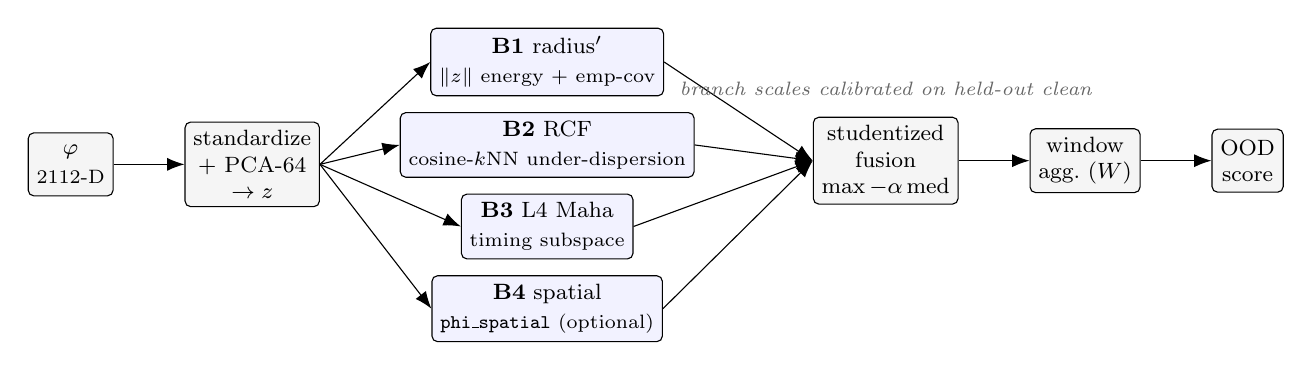
\begin{tikzpicture}[
    font=\footnotesize, >={Latex[length=2.2mm]}, node distance=4mm and 9mm,
    box/.style={draw, rounded corners=2pt, align=center, inner sep=3pt, minimum height=8mm, fill=black!4},
    br/.style={draw, rounded corners=2pt, align=center, inner sep=3pt, minimum height=7mm, fill=blue!5}]
    \node[box] (phi) {$\varphi$\\[1pt]\scriptsize 2112-D};
    \node[box, right=of phi] (proj) {standardize\\ $+$ PCA-64\\ $\to z$};
    \node[br, right=14mm of proj, yshift=13mm]  (b1) {\textbf{B1} radius$'$\\[1pt]\scriptsize $\lVert z\rVert$ energy $+$ emp-cov};
    \node[br, below=2mm of b1]  (b2) {\textbf{B2} RCF\\[1pt]\scriptsize cosine-$k$NN under-dispersion};
    \node[br, below=2mm of b2]  (b3) {\textbf{B3} L4 Maha\\[1pt]\scriptsize timing subspace};
    \node[br, below=2mm of b3]  (b4) {\textbf{B4} spatial\\[1pt]\scriptsize \texttt{phi\_spatial} (optional)};
    \node[box, right=15mm of b2, yshift=-2mm] (fuse) {studentized\\ fusion\\ $\max-\alpha\,\mathrm{med}$};
    \node[box, right=of fuse] (win) {window\\ agg.\ ($W$)};
    \node[box, right=of win] (out) {OOD\\ score};
    \draw[->] (phi) -- (proj);
    \foreach \b in {b1,b2,b3,b4} {\draw[->] (proj.east) -- (\b.west); \draw[->] (\b.east) -- (fuse.west);}
    \draw[->] (fuse) -- (win);
    \draw[->] (win) -- (out);
    \node[above=1.5mm of fuse, font=\scriptsize\itshape, text=black!60] {branch scales calibrated on held-out clean};
  \end{tikzpicture}}
  \caption{\textbf{The MDD pipeline} (described in Section~\ref{sec:mdd}): four two-sided
  branches over the PCA-denoised descriptor $z$, fused by a studentized $\max-\alpha\,\mathrm{median}$
  and optionally windowed.}
  \label{fig:mdd-flow}
\end{figure}

% =====================================================================
\section{Experimental Results}
\label{sec:results}

\subsection{Setup}
\label{sec:setup}
Prophesee Gen1 test split: $302$ sequences, $\approx343{,}099$ frames; each corruption applied per
whole sequence at L1--L5. Detectors are fit on clean-train frames only and are corruption-blind; the
split honours sequence boundaries so no clean frame appears in both fit and eval. We report AUROC
(AUPR / FPR@95\% at severity~5 in Table~\ref{tab:mdd-aupr}) per-frame and per-$W{=}64$-window; all
values are point estimates on a single split, with $95\%$ bootstrap CIs on the headline numbers in
Appendix~\ref{app:window}.

\subsection{Motivation: a pretrained detector degrades under event corruptions}
\label{sec:motivation}
We feed the pretrained hybrid SNN--ANN detector~\citep{ahmed2025hybrid} (clean
Gen1 test mAP $\approx0.36$, Table~\ref{tab:map-degradation}) each Gen1-C corruption with no
retraining, corrupting the event histogram before it is fed into the model.
\begin{table}[h]
  \centering
  \begin{minipage}[c]{0.55\linewidth}
  \centering\small
  \resizebox{\linewidth}{!}{%
  \begin{tabular}{lrrrrr}
    \toprule
    Corruption & S1 & S2 & S3 & S4 & S5 \\
    \midrule
    \texttt{hot\_pixel}         & 0.348 & 0.324 & 0.267 & 0.216 & 0.159 \\
    \texttt{event\_flood}       & 0.341 & 0.288 & 0.140 & 0.017 & 0.003 \\
    \texttt{temporal\_jitter}   & 0.353 & 0.348 & 0.344 & 0.333 & 0.302 \\
    \texttt{event\_rate\_shift} & 0.359 & 0.358 & 0.233 & 0.233 & 0.168 \\
    \texttt{polarity\_flip}     & 0.357 & 0.356 & 0.352 & 0.348 & 0.344 \\
    \texttt{spatial\_dropout}   & 0.357 & 0.351 & 0.344 & 0.323 & 0.265 \\
    \bottomrule
  \end{tabular}}
  \end{minipage}\hfill
  \begin{minipage}[c]{0.43\linewidth}
  \centering
  \includegraphics[width=\linewidth]{28_map_degradation.png}
  \end{minipage}
  \caption{Detection mAP (COCO AP@[.5:.95]) of the pretrained hybrid detector under each Gen1-C
  corruption at severities 1--5 (no retraining; clean baseline $0.358$), and the same data plotted
  (right). \texttt{event\_flood} degrades fastest; \texttt{polarity\_flip} stays flat despite being
  undetectable by the membrane.}
  \label{tab:map-degradation}
\end{table}
\texttt{event\_flood} is the most destructive (mAP $0.341\to0.003$); \texttt{polarity\_flip} is
nearly harmless ($-4\%$ at S5) and sits at AUROC $\approx0.43$ (Section~\ref{sec:limitations}).

\subsection{Main result: MDD OOD detection}
\label{sec:main}
Table~\ref{tab:mdd} reports fused MDD AUROC per corruption/severity,
per-frame~(a) and per-$64$-window~(b, $W{=}64$, ${\approx}0.64$\,s). One unsupervised,
corruption-blind score is already strong per frame on three of the six corruptions at severity~5;
aggregating over the bounded $64$-frame window (Section~\ref{sec:window}) brings a fourth,
\texttt{event\_flood}, past $0.85$ without whole-recording pooling. The two residuals are
theory-predicted (Section~\ref{sec:limitations}).

\begin{table}[t]
  \begin{minipage}[t]{0.49\linewidth}\centering\small
  {\footnotesize\textbf{(a) per-frame}}\\[2pt]
  \resizebox{\linewidth}{!}{%
  \begin{tabular}{lccccc}
    \toprule
    Corruption & S1 & S2 & S3 & S4 & S5 \\
    \midrule
    \texttt{hot\_pixel}        & 1.000 & 1.000 & 1.000 & 1.000 & 1.000 \\
    \texttt{temporal\_jitter}  & 0.658 & 0.700 & 0.742 & 0.799 & 0.850 \\
    \texttt{event\_rate\_shift}& 0.510 & 0.537 & 0.701 & 0.716 & 0.855 \\
    \texttt{spatial\_dropout}  & 0.500 & 0.501 & 0.502 & 0.517 & 0.560 \\
    \texttt{event\_flood}      & 0.504 & 0.509 & 0.517 & 0.531 & 0.551 \\
    \texttt{polarity\_flip}    & 0.504 & 0.508 & 0.516 & 0.527 & 0.540 \\
    \bottomrule
  \end{tabular}}
  \end{minipage}\hfill
  \begin{minipage}[t]{0.49\linewidth}\centering\small
  {\footnotesize\textbf{(b) per-$W{=}64$-window (${\approx}0.64$\,s)}}\\[2pt]
  \resizebox{\linewidth}{!}{%
  \begin{tabular}{lccccc}
    \toprule
    Corruption & S1 & S2 & S3 & S4 & S5 \\
    \midrule
    \texttt{hot\_pixel}        & 0.999 & 0.999 & 0.999 & 1.000 & 1.000 \\
    \texttt{temporal\_jitter}  & 0.679 & 0.731 & 0.759 & 0.816 & 0.869 \\
    \texttt{event\_rate\_shift}& 0.514 & 0.556 & 0.732 & 0.746 & 0.896 \\
    \texttt{event\_flood}      & 0.556 & 0.612 & 0.690 & 0.790 & 0.889 \\
    \texttt{spatial\_dropout}  & 0.500 & 0.513 & 0.502 & 0.521 & 0.576 \\
    \texttt{polarity\_flip}    & 0.514 & 0.537 & 0.543 & 0.563 & 0.579 \\
    \bottomrule
  \end{tabular}}
  \end{minipage}
  \caption{Fused MDD AUROC (shipped improved default: \texttt{radius}$'$ + studentized fusion).
  \textbf{(a)}~per-frame: contractions and the invariant \texttt{polarity\_flip} sit near chance.
  \textbf{(b)}~per-$W{=}64$-window: four corruptions reach ${\geq}0.85$ without full-recording
  pooling; \texttt{spatial\_dropout} and \texttt{polarity\_flip} remain the residuals.}
  \label{tab:mdd}\label{tab:mdd-frame}\label{tab:mdd-w64}
\end{table}

\subsection{Efficient MDD}
\label{sec:efficient-mdd}
The result above still scores against the full $204{,}096$-frame clean reference with a hard
top-$64$ cosine search. To make MDD deployable on-device, we shrink the reference to $200$ points
chosen by farthest-point sampling (far better than random subsampling at matched size) and replace
the hard top-$k$ search with a $\mathrm{TopK}$-free softmax-weighted average, since embedded ONNX
toolchains commonly reject $\mathrm{TopK}$. This costs only $0.010$ mean AUROC ($0.802\to0.792$).
We exported the resulting model with static shapes and measured real (not simulated) latency on
phone-class NPUs/CPUs and two Arm Cortex-M7 microcontrollers: phone-class devices clear the
$50$\,ms/frame real-time deadline by a wide margin (under $1$\,ms), and one of the two MCU boards
does too ($34.93$\,ms on the STM32H7S78-DK), but the other (STM32H735G-DK, a slightly slower
$550$\,MHz core) comes in at $52.42$\,ms and \emph{misses} the deadline (Table~\ref{tab:mdd-hw}) ---
board-level differences, not just clock speed, decide whether a bare Cortex-M7 clears real-time on
this workload. The exported graph takes both $\varphi$ ($2112$-D) and \texttt{phi\_spatial}
($1408$-D) per frame and, per ST Edge AI Core's static analysis, costs $2.65$M MACCs, $30.06$\,KiB
of RAM, and $10.03$\,MiB of flash --- $15$--$18\times$ under either board's available internal RAM,
with the flash placed in the external flash both boards carry. We did not separately profile a
\texttt{phi\_spatial}-free variant on hardware, so the reported cost is for the full (spatial-branch
included) model; isolating the spatial branch's incremental on-device delta is future work. Full
derivation and the reference-reduction ablation are in Appendix~\ref{app:compute}.

\begin{table}[t]
  \centering\small
  \caption{Measured (not simulated) inference latency of the embedded MDD variant on real
  hardware, against the $50$\,ms/frame deadline. Phone-class devices measured via Qualcomm AI
  Hub~\citep{qualcommaihub}; the STM32 board via ST Edge AI Developer Cloud's~\citep{stedgeai}
  hardware farm.}
  \label{tab:mdd-hw}
  \begin{tabular}{llcc}
    \toprule
    Device & Compute unit & Class & Measured latency \\
    \midrule
    Samsung Galaxy S24  & NPU & phone SoC & $0.137$\,ms \\
    Samsung Galaxy S24  & CPU & phone SoC & $0.101$\,ms \\
    Samsung Galaxy A14 5G & CPU & phone SoC (budget) & $0.823$\,ms \\
    Google Pixel 3a     & CPU & phone SoC (oldest tested) & $1.091$\,ms \\
    STM32H7S78-DK       & CPU & MCU, Arm Cortex-M7 @ 600\,MHz & $34.93$\,ms \\
    STM32H735G-DK       & CPU & MCU, Arm Cortex-M7 @ 550\,MHz & $52.42$\,ms$^\dagger$ \\
    \bottomrule
  \end{tabular}

  \vspace{2pt}
  {\scriptsize $^\dagger$ The one board tested that \emph{misses} the $50$\,ms/frame deadline
  ($1.048\times$ over budget).}
\end{table}

\subsection{The geometry of corruption}
\label{sec:geometry}
Figure~\ref{fig:geometry} shows the geometry underlying Section~\ref{sec:theory}. Membrane
energy $\lVert z\rVert$ moves \emph{right} for dilations and \emph{left} for contractions
(Figure~\ref{fig:geometry}a); the Mahalanobis $d^2$ of the contractions sits at \emph{smaller}
values than clean (Figure~\ref{fig:geometry}b), the AUROC$<0.5$ inversion; and
the clean$\to$corrupt centroid drift in a shared clean-PCA separates
the corruption directions, with the two dilations (\texttt{hot\_pixel}, \texttt{event\_flood};
cosine $0.75$) and the two contraction-side residuals (\texttt{polarity\_flip},
\texttt{spatial\_dropout}; $0.73$) each sharing a direction. Figure~\ref{fig:geometry}
(radial energy and Mahalanobis $d^2$) and the PCA drift-arrow/cosine views are both in
Appendix~\ref{app:extra-figs}.

\subsection{Representation ablation: which signal from the forward pass?}
\label{sec:repr-ablation}
The geometry above operates on full membrane $\varphi=[\mu,\sigma^2,\kappa]$.
We also check whether a cheaper slice of $\varphi$, or a different signal from the
\emph{same} forward pass, could substitute: no single moment or alternative read-out (spike-rate,
spike-entropy, ANN features, cls-head features) matches full membrane, each dropping a specific
corruption's signal (e.g.\ spike-rate is blind to sub-threshold shifts, Example~\ref{prop:spike}).
Full membrane wins overall (mean AUROC $0.572$); full per-corruption breakdown
and methodology in Appendix~\ref{app:repr} (Table~\ref{tab:repr-ablation}).

\begin{figure}[t]
  \centering
  \includegraphics[width=0.62\linewidth]{31_repr_mean_summary.png}
  \caption{\textbf{Representation ablation}, mean AUROC over all corruptions and severities.
  Full membrane $\varphi$ leads; ANN features are the weakest read-out from the same forward
  pass. Per-corruption breakdown in Appendix~\ref{app:repr}.}
  \label{fig:repr-summary}
\end{figure}

\subsection{Branch decomposition and fusion ablation}
\label{sec:branches}
Figure~\ref{fig:branches}a shows each branch is corruption-specialized (radius owns dilations, L4
owns timing, RCF/spatial own contractions); the plain calibrated \texttt{max} sits \emph{below}
the best single branch on both residuals, motivating the studentized fusion
(Appendix~\ref{app:mdd-improve}). This follows the classical outlier-ensemble bias--variance
argument~\citep{aggarwal2015ensembles}: when an anomaly is flagged by only a \emph{few} base
detectors (here, one branch per corruption; leave-one-out, Table~\ref{tab:mdd-loo}), averaging or
consensus combiners are the wrong regime --- they dilute the one branch that fired --- and a
variance-corrected \texttt{max} is the theoretically preferred aggregator; our 16-combiner benchmark
(Appendix~\ref{app:fusion}) confirms this empirically, with every averaging/consensus/
rank-aggregation/copula combiner underperforming the \emph{max} family. Folding an empirical-covariance Mahalanobis into the radius
branch and replacing \texttt{max} with $\max-\alpha\cdot\mathrm{median}$
recovers \texttt{spatial\_dropout} from its plain-\texttt{max}
baseline to $0.620$ per sequence ($0.576$ at $W{=}64$) and lifts the worst-corruption floor with no
easy-corruption regression, though still short of the \texttt{rcf} branch's own $0.693$ ceiling
(Table~\ref{tab:mdd-branch}); pushing $\alpha$ further approaches that ceiling ($0.689$) only by
trading away \texttt{polarity\_flip} (Appendix~\ref{app:mdd-improve}, Figure~\ref{fig:alpha-tradeoff}a).

\subsection{Windowed aggregation: the deployable operating point}
\label{sec:window}
Table~\ref{tab:mdd-w64} (main text) is the headline: $W{=}64$ (${\approx}0.64$\,s per decision)
recovers most of the signal \emph{without} any whole-recording assumption; full-sequence aggregation
(${\sim}730$ frames, once per recording) is an optimistic upper bound (Appendix~\ref{app:window},
Table~\ref{tab:window}). The $W$ sweep at severity~5 shows when the signal becomes reliable:
\texttt{hot\_pixel} is at $1.00$ by $W{=}16$ (${\approx}0.16$\,s), all four detectable corruptions
exceed $0.85$ by $W{=}64$, and \texttt{event\_flood} reaches $0.98$ by $W{=}128$.

\paragraph{Windowing versus per-frame signal.} \texttt{event\_flood}'s rise ($0.55\!\to\!0.98$) comes
from integrating a temporally-consistent bias, so we report the \emph{windowed} value.
\texttt{polarity\_flip} and \texttt{spatial\_dropout} stay flat at every window: pooling cannot recover
a per-frame signal that is not there.

\begin{figure}[t]
  \centering
  \includegraphics[width=\linewidth]{40_branch_window.png}
  \caption{MDD detection at L5. \textbf{(a)}~per-branch AUROC (corruption $\times$ branch, $W{=}64$):
  each branch owns a different corruption and \texttt{fused} tracks the per-corruption best.
  \textbf{(b)}~fused AUROC vs.\ aggregation window $W$: the four detectable corruptions rise with $W$
  (\texttt{event\_flood} slowest, crossing $0.85$ near $W{=}128$) while the two residuals stay flat at
  \emph{every} window. The $\alpha$ trade-off is in Appendix~\ref{app:mdd-improve}
  (Figure~\ref{fig:alpha-tradeoff}a); the combiner benchmark is in Appendix~\ref{app:fusion}.}
  \label{fig:branches}
  \label{fig:detect}
  \label{fig:window}
\end{figure}

% =====================================================================
\section{Limitations and the Open Challenge}
\label{sec:limitations}

\paragraph{Residuals.}
Two corruptions remain near chance when detected from the membrane alone, but for different reasons,
and across these six corruptions how detectable a corruption is tracks how much harm it does.
\texttt{spatial\_dropout} causes real harm ($-26\%$ mAP at S5, Section~\ref{sec:motivation}) but
leaves no per-frame membrane signature, because that signature is \emph{spatial} and global average
pooling throws spatial layout away. The spatial-dispersion features we release
(\texttt{phi\_spatial}) feed MDD's spatial branch, and we validated end-to-end that they do recover
this signal on a controlled test case (a signal present only in \texttt{phi\_spatial} lifts AUROC
from $\approx0.50$, without the spatial branch, to $\approx1.00$; Appendix~\ref{app:spatial-check}).
So this is a genuine \textbf{open problem}: a harmful corruption with no cheap per-frame signal, and
the gap is capped by a provable ceiling on any $\varphi$-based detector, not just a tuning failure:
no score computed from $\varphi$ can exceed $\mathrm{AUROC}\le\tfrac12+\delta$, where $\delta$ is the
total variation distance between the clean and corrupted $\varphi$ distributions
(Proposition~\ref{prop:tv-ceiling}). \texttt{polarity\_flip} is a different case: a property of the
trained network's polarity invariance, not of our representation. It causes negligible harm
($-4\%$ at S5) and cannot be detected from $V_{\mathrm{mem}}$ by construction, since the model itself
is unaffected: the same network invariance that makes a corruption harmless also makes it
invisible to $\varphi$, separating \texttt{polarity\_flip} (an invariance) from
\texttt{spatial\_dropout} (harmful but hidden by the pooling blind spot instead); see
Proposition~\ref{prop:invariance}.

\paragraph{Other limitations.}
(i)~The low-compute claim is only about the \emph{signal}, not the MDD detector that scores it
(host-side cost profiled in \S\ref{sec:efficient-mdd}, Appendix~\ref{app:compute}); notably, the
reference-set reduction there lands almost entirely on \texttt{spatial\_dropout}
($-0.106$, Table~\ref{tab:mdd-reduce}) -- shrinking MDD for deployment makes the open problem
above worse, not better.
(ii)~$\varphi$ is read from the membrane state including the reset that follows each spike, so the
linear, sub-threshold theory in Section~\ref{sec:theory} is only an approximation; a version of $V$
with spikes strictly excluded, and a reset-aware analysis, remain untested.
(iii)~Our AUROC values are point estimates from a single data split; we report $95\%$ bootstrap
confidence intervals (resampling recordings) for the headline numbers in Appendix~\ref{app:window}.
(iv)~We use a single dataset (Gen1) and a single pretrained host model; transfer to other datasets
(DSEC, Gen4) or architectures is untested. The corruption severities are synthetic, monotone
transforms chosen to resemble real sensor faults (Section~\ref{sec:corruptions},
Appendix~\ref{app:mechanisms}), but they are \emph{not} calibrated against measured hardware faults;
a realistic-noise simulator such as v2e~\citep{hu2021v2e}, or capturing faults directly from hardware,
would validate this mapping. What we contribute here is the benchmark, protocol, and feature release.
(v)~The headline numbers use a $64$-frame window (Table~\ref{tab:mdd-w64}); the full-recording upper
bound (Table~\ref{tab:window}) should not be read as a per-frame detection rate. AUROC measures how
separable clean and corrupted scores are once the ground-truth labels are known, not a value the
detector would reproduce at a fixed deployment threshold, where no such labels are available.

\section{Conclusion}
\label{sec:conclusion}
Gen1-C, the leaky-integrator theory, and MDD together turn a signal that costs nothing extra to
read into a detector whose successes and residuals are both predicted in advance rather than
discovered post hoc. The one open problem, \texttt{spatial\_dropout}, points to spatial-dispersion
features and adaptive neurons as the natural next directions.

% =====================================================================
\bibliography{refs}
\bibliographystyle{iclr2025_conference}

% =====================================================================
% APPENDIX -- the full experimental record ("everything we tried").
% =====================================================================
\appendix
\section*{Appendix}
\addcontentsline{toc}{section}{Appendix}

\noindent This appendix documents the complete experimental program -- including the levers that
did \emph{not} work -- so the headline claims can be audited against everything we tried.

\section{Implementation, Splits, and Reproducibility}
\label{app:impl}

\paragraph{Feature extraction.} A forward hook on all four
parametric LIF layers ($64/128/256/256$, $704$ channels) captures
$V\in\mathbb{R}^{T\times1\times C\times H\times W}$, GAPs over space, and reduces to
$[\mu,\sigma^2,\kappa]$ per channel ($\varphi$, $2112$-D). \texttt{phi\_spatial} ($1408$-D) adds
per-channel spatial variance and participation ratio, stored \texttt{float32} (\texttt{float16}
overflows the spatial-variance channel under \texttt{event\_flood}).

\paragraph{Protocol.} Metrics AUROC, AUPR, FPR@95\%, per-frame and per-sequence, with $95\%$ bootstrap
CIs on the headline numbers (Appendix~\ref{app:window}).

\begin{table}[H]
  \centering\small
  \begin{tabular}{lcccc}
    \toprule
    & \multicolumn{2}{c}{per-frame} & \multicolumn{2}{c}{per-$W{=}64$-window} \\
    \cmidrule(lr){2-3}\cmidrule(lr){4-5}
    Corruption (S5) & AUPR & FPR@95\% & AUPR & FPR@95\% \\
    \midrule
    \texttt{hot\_pixel}        & 1.000 & 0.000 & 1.000 & 0.000 \\
    \texttt{temporal\_jitter}  & 0.867 & 0.657 & 0.893 & 0.678 \\
    \texttt{event\_rate\_shift}& 0.862 & 0.685 & 0.913 & 0.641 \\
    \texttt{event\_flood}      & 0.603 & 0.944 & 0.928 & 0.767 \\
    \texttt{spatial\_dropout}  & 0.551 & 0.944 & 0.571 & 0.940 \\
    \texttt{polarity\_flip}    & 0.548 & 0.936 & 0.589 & 0.933 \\
    \bottomrule
  \end{tabular}
  \caption{Fused MDD at severity~5: AUPR and FPR@95\%, per-frame and per-$W{=}64$-window, computed
  from the same fitted branches and studentized fusion as Table~\ref{tab:mdd} (whose S5 AUROC
  column applies unchanged here).}
  \label{tab:mdd-aupr}
\end{table}

\paragraph{Reproduction budget.} The one-time GPU cost is extraction ($\sim\!90$--$150$\,GB of
$\varphi$); every downstream stage then runs on $\varphi$ directly in minutes to an hour on one GPU.

\section{Monotonicity Theory: Statements and Proofs}
\label{app:theory}

We make the qualitative predictions of Section~\ref{sec:theory} \emph{quantitative}.
Let severity be $\gamma\ge0$ and model a corruption family as an additive drift on the
per-layer input current:
\begin{equation}
  X_t(\gamma) = X_t(0) + \gamma\Delta_t + \epsilon_t(\gamma),\qquad \mathbb{E}[\epsilon_t]=0.
  \label{eq:drift-model}
\end{equation}
Writing the membrane deviation $\delta V_t(\gamma)=V_t(\gamma)-V_t(0)$ and linearising the
PLIF update $V[t]=(1-\tfrac1\tau)V[t-1]+WX[t]$ in the sub-threshold regime (bounded reset
mismatch) gives
\begin{equation}
  \delta V_t(\gamma) = \lambda\,\delta V_{t-1}(\gamma)+W\!\left(\gamma\Delta_t+\epsilon_t\right),
  \label{eq:linearized}
\end{equation}
which unrolls to
\begin{equation}
  \delta V_t(\gamma) = \sum_{k=0}^{t}\lambda^{\,t-k}W\!\left(\gamma\Delta_k+\epsilon_k\right).
  \label{eq:unroll-dev}
\end{equation}
Everything below is one of two kinds of result: how this linear recursion propagates a monotone
perturbation (Lemma~\ref{lem:linresponse}, Corollaries~\ref{thm:drift}--\ref{thm:score}), or how much
information the membrane retains relative to the spikes it produces (Lemma~\ref{lem:dpi-general},
Corollaries~\ref{prop:dpi}--\ref{cor:rate-dpi} and Proposition~\ref{prop:moment-bound}). The reset
nonlinearity both families treat as a bounded perturbation is quantified first.

\paragraph{Reset-aware dynamics and the error term $R_t$.} The linearisation~\eqref{eq:linearized} is
\emph{exact between spikes}; the sole nonlinearity is the hard reset, which subtracts the threshold
$\theta$ from the trajectory at each emission. With the spike indicator $s_t=\mathbf{1}[V_t\ge\theta]$
the reset-aware recurrence is
\begin{equation}
  V[t] = \Bigl(1-\tfrac1\tau\Bigr)V[t-1] + WX[t] - \theta\, s_{t-1},
  \label{eq:reset-recurrence}
\end{equation}
so the membrane deviation $\delta V_t$ of~\eqref{eq:unroll-dev} acquires exactly one extra,
\emph{impulsive} term, the difference of the two reset trains:
\begin{equation}
  R_t = -\,\theta\sum_{k=0}^{t}\lambda^{\,t-k}\bigl(s_k^{\mathrm{OOD}}-s_k^{\mathrm{ID}}\bigr),
  \qquad \lambda := 1-\tfrac1\tau .
  \label{eq:reset-term}
\end{equation}
This is the PLIF nonlinearity written out, not a small-signal approximation: the dynamics are a
\emph{piecewise-linear hybrid system}, linear on inter-spike intervals plus a bounded jump at each
reset. The jump term is controlled by the firing statistics.
\begin{theorem}[Reset error scales with the firing rate]
\label{lem:reset}
Let $\rho_\Delta=\sup_k\Pr[\,s_k^{\mathrm{OOD}}\neq s_k^{\mathrm{ID}}\,]$ be the per-step probability
that the clean and corrupted spike trains disagree. Then
\begin{equation}
  \mathbb{E}\,|R_t|\;\le\;\frac{\theta\,\rho_\Delta}{1-\lambda}.
  \label{eq:reset-bound}
\end{equation}
In particular $\rho_\Delta=0$ in the sub-threshold regime, recovering $R_t\equiv0$ and the exact
linear results below, and the membrane-mean signal $b$ of Corollary~\ref{thm:drift} dominates the reset
error whenever $|b|\gg\theta\rho_\Delta/(1-\lambda)$.
\end{theorem}
\begin{proof}
By the triangle inequality $|R_t|\le\theta\sum_{k=0}^{t}\lambda^{\,t-k}\,|s_k^{\mathrm{OOD}}-s_k^{\mathrm{ID}}|$.
Taking expectations and using $\mathbb{E}\,|s_k^{\mathrm{OOD}}-s_k^{\mathrm{ID}}|
=\Pr[s_k^{\mathrm{OOD}}\neq s_k^{\mathrm{ID}}]\le\rho_\Delta$ and the geometric sum
$\sum_{k\le t}\lambda^{\,t-k}\le(1-\lambda)^{-1}$ gives~\eqref{eq:reset-bound}.
\end{proof}
\noindent Theorem~\ref{lem:reset} makes the ``bounded reset mismatch'' assumption of
Corollaries~\ref{thm:drift}--\ref{thm:score} \emph{quantitative}: the constant $C_R$ is
$\theta\rho_\Delta/(1-\lambda)$, the guarantees are exact in the low-firing regime where the membrane
signal is most distinctive, and they degrade gracefully, linearly in the firing-disagreement rate
$\rho_\Delta$, as neurons fire and reset more often.

\subsection{Linear-response monotonicity}
\label{app:theory-linresponse}

The next four results are all instances of one fact: a stable linear recursion (or, one level up, a
quadratic form of a linearly-drifting feature vector) turns a monotone perturbation of its input into
a monotone perturbation of its output. Stating that fact once, as a lemma, lets each corollary below
be a two-line specialization rather than a repeated derivation.

\begin{lemma}[Linear-response monotonicity]
\label{lem:linresponse}
\textbf{(a) Membrane moments.} Let $\delta V_t(\gamma)$ solve the linearised PLIF
recursion~\eqref{eq:unroll-dev} for a per-channel current whose mean or covariance is affine in
$\gamma$: either $\mathbb{E}[\Delta_k]\neq0$ under~\eqref{eq:drift-model} (mean-drift), or
\begin{equation}
  \mathrm{Cov}(X_t(\gamma)) = \Sigma_0+\gamma\Sigma_\Delta, \qquad \Sigma_\Delta\succeq0
  \label{eq:var-assumption}
\end{equation}
(covariance-inflation). Then, up to the bounded reset error $R_t$ of Theorem~\ref{lem:reset},
\begin{align}
  \mathbb{E}[\delta V_t(\gamma)] &= \gamma\sum_{k=0}^{t}\lambda^{\,t-k}W\,\mathbb{E}[\Delta_k] + R_t,
    &&\text{monotone in }\gamma\text{ whenever the sum}\neq0, \label{eq:lin-mean}\\
  \Sigma_V(\gamma) &= \frac{W^2}{1-\lambda^2}\bigl(\Sigma_0+\gamma\Sigma_\Delta\bigr),
    &&\frac{d}{d\gamma}\mathrm{tr}\,\Sigma_V(\gamma) = \frac{W^2\,\mathrm{tr}(\Sigma_\Delta)}{1-\lambda^2}\ge0.
  \label{eq:lin-var}
\end{align}
\textbf{(b) Any linearly-drifting quadratic form.} Let $z_\gamma$ be a feature vector with
\begin{equation}
  \mathbb{E}[z_\gamma] = m_0+\gamma b, \qquad \mathrm{Cov}(z_\gamma) = C_0+\gamma C_\Delta,
  \qquad C_\Delta\succeq0.
  \label{eq:linresponse-assumptions}
\end{equation}
Then for the quadratic form $D^2(z_\gamma) := (z_\gamma-m_0)^\top C_0^{-1}(z_\gamma-m_0)$,
\begin{equation}
  \mathbb{E}\bigl[D^2(z_\gamma)\bigr] = n + \gamma\,\mathrm{tr}(C_0^{-1}C_\Delta) + \gamma^2\,b^\top C_0^{-1}b,
  \label{eq:lin-quad}
\end{equation}
non-decreasing in $\gamma\ge0$ and strictly increasing whenever $b\neq0$ or $C_\Delta\neq0$.
\end{lemma}
\begin{proof}
\textbf{(a)} Taking expectations in~\eqref{eq:unroll-dev} with $\mathbb{E}[\epsilon_k]=0$ gives the
first line of~\eqref{eq:lin-mean} directly, with $R_t$ collecting the reset-mismatch error
($|R_t|\le C_R$ in the sub-threshold regime). For~\eqref{eq:lin-var}, model each channel as a stable
AR(1) process $V[t]=\lambda V[t-1]+WX[t]$; at stationarity the variance solves the discrete Lyapunov
equation $\Sigma_V=\lambda^2\Sigma_V+W^2\Sigma_X$, i.e.\ $\Sigma_V=W^2\Sigma_X/(1-\lambda^2)$.
Substituting $\Sigma_X=\Sigma_0+\gamma\Sigma_\Delta$ and differentiating the trace gives
$\mathrm{tr}(\Sigma_\Delta)\ge0\Rightarrow d/d\gamma\,\mathrm{tr}\,\Sigma_V(\gamma)\ge0$.
\textbf{(b)} Write $z_\gamma=m_0+\gamma b+\xi_\gamma$ with $\mathbb{E}[\xi_\gamma]=0$,
$\mathrm{Cov}(\xi_\gamma)=C_0+\gamma C_\Delta$. Expanding the quadratic form,
\begin{align*}
  \mathbb{E}\bigl[D^2(z_\gamma)\bigr]
  &= \mathbb{E}\bigl[(\gamma b+\xi_\gamma)^\top C_0^{-1}(\gamma b+\xi_\gamma)\bigr] \\
  &= \gamma^2\,b^\top C_0^{-1}b + \underbrace{2\gamma\,b^\top C_0^{-1}\mathbb{E}[\xi_\gamma]}_{=\,0}
     + \mathbb{E}\bigl[\xi_\gamma^\top C_0^{-1}\xi_\gamma\bigr] \\
  &= \gamma^2\,b^\top C_0^{-1}b + \mathrm{tr}\bigl(C_0^{-1}(C_0+\gamma C_\Delta)\bigr)
   = n + \gamma\,\mathrm{tr}(C_0^{-1}C_\Delta) + \gamma^2\,b^\top C_0^{-1}b,
\end{align*}
using the trace identity $\mathbb{E}[\xi^\top A\xi]=\mathrm{tr}(A\,\mathrm{Cov}(\xi))$ for zero-mean
$\xi$. Both coefficients are non-negative ($C_0^{-1}\succ0$, $C_\Delta\succeq0$, so
$\mathrm{tr}(C_0^{-1}C_\Delta)\ge0$ and $b^\top C_0^{-1}b\ge0$), giving~\eqref{eq:lin-quad}.
\end{proof}

\begin{corollary}[Monotone membrane drift]
\label{thm:drift}
Under~\eqref{eq:drift-model} with $\mathbb{E}[\Delta_k]\neq0$ in at least one monitored PLIF layer
and bounded reset mismatch, Lemma~\ref{lem:linresponse}(a)/\eqref{eq:lin-mean} gives
\begin{equation}
  \mathbb{E}[\delta V_t(\gamma)] = \gamma\,b + R_t, \qquad
  b := \sum_{k=0}^{t}\lambda^{\,t-k}W\,\mathbb{E}[\Delta_k], \qquad |R_t|\le C_R.
  \label{eq:drift-result}
\end{equation}
The temporal-mean coordinate $\mu$ of $\varphi$ is therefore OOD-informative whenever $b\neq0$.
\end{corollary}

\begin{corollary}[Monotone membrane variance]
\label{thm:var}
Under the covariance-inflation hypothesis~\eqref{eq:var-assumption}, Lemma~\ref{lem:linresponse}(a)/
\eqref{eq:lin-var} gives a stationary membrane covariance $\Sigma_V(\gamma)$ whose trace is
non-decreasing in $\gamma$. Any corruption that increases the input covariance in the PSD order
therefore monotonically increases the membrane variance, justifying the $\sigma^2$ and $\kappa$
coordinates of $\varphi$ beyond the mean.
\end{corollary}

\begin{corollary}[Marginal-preserving reordering shifts membrane variance]
\label{thm:jitter}
Let a corruption $T_\gamma$ permute event timing within a bounded window, leaving the per-bin
marginal mean and variance $m,s^2$ unchanged but perturbing the input autocovariance
$\gamma(j)\to\gamma(j)+\Delta\gamma(j)$ for $j\ge1$. Channeling the perturbation of
Lemma~\ref{lem:linresponse}(a) through the autocovariance term of the steady-state
variance~\eqref{eq:moments} rather than $\Sigma_0$ directly, the membrane variance shifts by
\begin{equation}
  \Delta\,\mathrm{Var}[V] = \frac{2W^2}{1-\lambda^2}\sum_{j\ge1}\Delta\gamma(j)\,\lambda^{j},
  \label{eq:jitter-shift}
\end{equation}
whose magnitude is monotone increasing in $\lambda=1-1/\tau$ for every fixed $j$: deeper layers
(larger $\tau$) amplify the same autocovariance perturbation into a larger $\sigma^2$ shift, even
though the input's marginal moments are unchanged.
\end{corollary}
\begin{proof}
Since $m,s^2$ are held fixed by construction, only the autocovariance term changes under $T_\gamma$,
giving~\eqref{eq:jitter-shift} directly by linearity. Differentiating the $j$-th summand's
coefficient with respect to $\lambda$,
\begin{equation*}
  \frac{d}{d\lambda}\frac{\lambda^{j}}{1-\lambda^2}
  = \frac{\lambda^{j-1}\bigl[j+(2-j)\lambda^2\bigr]}{(1-\lambda^2)^2},
\end{equation*}
and the bracket is affine in $\lambda^2$ with value $j>0$ at $\lambda^2=0$ and value $2>0$ at
$\lambda^2=1$, hence strictly positive throughout $\lambda\in(0,1)$ for every integer $j\ge1$: each
term of~\eqref{eq:jitter-shift} is strictly increasing in $\lambda$.
\end{proof}

\begin{corollary}[MP-OOD score monotonicity]
\label{thm:score}
Let the clean calibration model be $(m_0,C_0)$ and suppose $\varphi_\gamma$ satisfies the
$z_\gamma=\varphi_\gamma$ instance of~\eqref{eq:linresponse-assumptions}:
\begin{equation}
  \mathbb{E}[\varphi_\gamma] = m_0+\gamma b,\qquad
  \mathrm{Cov}(\varphi_\gamma) = C_0+\gamma C_\Delta,\quad C_\Delta\succeq0.
  \label{eq:score-assumptions}
\end{equation}
By Lemma~\ref{lem:linresponse}(b)/\eqref{eq:lin-quad}, the expected Mahalanobis OOD score
$D^2(\varphi_\gamma)=(\varphi_\gamma-m_0)^\top C_0^{-1}(\varphi_\gamma-m_0)$ satisfies
\begin{equation}
  \mathbb{E}\!\left[D^2(\varphi_\gamma)\right]
  = n + \gamma\,\mathrm{tr}(C_0^{-1}C_\Delta) + \gamma^2\,b^\top C_0^{-1}b,
  \label{eq:score-mono}
\end{equation}
non-decreasing in $\gamma\ge0$, strictly increasing whenever $b\neq0$ or $C_\Delta\neq0$. The lone
measured exception, \texttt{spatial\_dropout} ($\rho=-1$), is the failure
of~\eqref{eq:score-assumptions} when GAP pools away the dimension in which $b$ lives: the score then
sees only a contraction toward $m_0$ and the sign flips.
\end{corollary}

\subsection{Data-processing dominance of the membrane over spike statistics}
\label{app:theory-dpi}

The next results are all instances of a second shared fact: if a statistic is a deterministic
function of a richer object, the data-processing inequality bounds how much it can know about any
external parameter relative to that richer object.

\begin{lemma}[Data-processing dominance]
\label{lem:dpi-general}
Let $Y=h(Z)$ for a deterministic, measurable map $h$, and let $\gamma$ be any parameter (or label)
with a prior. Then for any post-hoc statistic $g$,
\begin{equation}
  I\bigl(\gamma;\,g(Y)\bigr) \;\le\; I\bigl(\gamma;\,Y\bigr) \;\le\; I\bigl(\gamma;\,Z\bigr),
  \label{eq:dpi-general}
\end{equation}
with equality on the right iff $\gamma\perp Z\mid Y$.
\end{lemma}
\begin{proof}
$Y=h(Z)$ makes $\gamma\to Z\to Y$ Markov, so the data-processing inequality gives
$I(\gamma;Y)\le I(\gamma;Z)$; applying it again to the further map $g$ gives the left inequality.
Equality holds iff $\gamma\to Y\to Z$ is also Markov, i.e.\ $Z\perp\gamma\mid Y$.
\end{proof}

\begin{corollary}[Membrane information dominates spikes in every regime]
\label{prop:dpi}
The spike train is a deterministic function of the membrane trajectory,
$s_{1:T}=h(V_{1:T})$ with $h(v)_t=\mathbf{1}[v_t\ge\theta]$. Instantiating
Lemma~\ref{lem:dpi-general} with $Z=V_{1:T}$, $Y=s_{1:T}$, for any post-hoc spike statistic $g$,
\begin{equation}
  I\bigl(\gamma;\,g(s_{1:T})\bigr)\;\le\;I\bigl(\gamma;\,s_{1:T}\bigr)\;\le\;I\bigl(\gamma;\,V_{1:T}\bigr).
  \label{eq:dpi}
\end{equation}
A membrane-based detector therefore has at least as much information about the corruption as
\emph{any} spike-count detector, with strict gain whenever the corruption perturbs the membrane
other than through threshold crossings.
\end{corollary}

\begin{example}[Sub-threshold shifts are invisible to spike counts]
\label{prop:spike}
Concretely: a neuron with threshold $\theta$, in-distribution potential in $[0,\theta-\varepsilon]$,
and a corruption shifting every membrane value by $0<\delta<\varepsilon$. Then
\begin{equation}
  V^{\mathrm{OOD}}_t = V^{\mathrm{ID}}_t+\delta \;\le\;\theta-\varepsilon+\delta\;<\;\theta,
  \label{eq:spike-example}
\end{equation}
so neither trajectory fires ($s_t^{\mathrm{ID}}=s_t^{\mathrm{OOD}}=0$ for all $t$) and every
spike-count detector assigns identical scores to the two distributions. Yet by linearity of
expectation $\bar V^{\mathrm{OOD}}-\bar V^{\mathrm{ID}}=\delta$, so a membrane-potential detector
(e.g., Mahalanobis on $\varphi$) separates them directly: sub-threshold membrane OOD strictly
subsumes spike-count OOD. This is the equality case of Corollary~\ref{prop:dpi} being tight
($I(\gamma;s_{1:T})=0<I(\gamma;V_{1:T})$), not a separate argument.
\end{example}

\noindent This holds under resets, nonlinearities, and arbitrary firing rates: spiking is a lossy
coarsening of the membrane. One scope caveat: the bound orders the \emph{full} trajectory
$V_{1:T}$; the deployed $\varphi$ is itself a lossy map of $V$, so Lemma~\ref{lem:dpi-general} does
not by itself order $\varphi$ against spikes -- the next result closes that gap under a stationarity
hypothesis. $\varphi$-dominance is provable for the sub-threshold-shift family
(Example~\ref{prop:spike}) and, under the stationary model, for \emph{every rate-based} spike
statistic (Corollary~\ref{cor:rate-dpi}); only against statistics exploiting temporal structure
beyond the marginal is it \emph{empirical} (Appendix~\ref{app:repr}: $\varphi$ mean AUROC $0.572$ vs
spike-rate $0.537$). Corollaries~\ref{thm:drift}--\ref{thm:score} additionally assume
stationarity and the bounded reset mismatch of Theorem~\ref{lem:reset}.

\begin{corollary}[$\varphi$ dominates rate-based spike statistics under location--scale]
\label{cor:rate-dpi}
Adopt the wide-sense-stationary membrane model of Corollaries~\ref{thm:drift}--\ref{thm:var} and
suppose each PLIF unit's sub-threshold potential is \emph{location--scale}:
$V_t\overset{d}{=}\mu+\sigma Z$ for a fixed standardized law $Z\sim F_0$ (mean $0$, variance $1$),
with $(\mu,\sigma^2)$ the coordinates $\varphi$ records. Then the mean firing rate is a deterministic
function of $\varphi$,
\begin{equation}
  r \;=\; \Pr[V_t\ge\theta] \;=\; \bar F_0\!\Big(\tfrac{\theta-\mu}{\sigma}\Big)\;=\;h(\varphi),
  \qquad \bar F_0:=1-F_0,
  \label{eq:rate-of-phi}
\end{equation}
so instantiating Lemma~\ref{lem:dpi-general} with $Z=\varphi$, $Y=r=h(\varphi)$, for any post-hoc
rate statistic $g$ -- in particular the spike-rate $r$ itself and the spike-entropy
$H(r)=-r\log r-(1-r)\log(1-r)$ --
\begin{equation}
  I\bigl(\gamma;\,g(r)\bigr)\;\le\;I\bigl(\gamma;\,r\bigr)\;\le\;I\bigl(\gamma;\,\varphi\bigr).
  \label{eq:phi-rate-dpi}
\end{equation}
The right inequality is \emph{strict} whenever $\gamma$ moves $(\mu,\sigma)$ off a level set of
$(\theta-\mu)/\sigma$ (e.g.\ the variance/kurtosis inflation of \texttt{temporal\_jitter} at
$\mu\!\approx\!\text{const}$), which leaves every rate statistic fixed while moving $\varphi$. The
Gaussian marginal of Corollary~\ref{thm:var} is the special case $F_0=\Phi$; the hypothesis needed is
only that a fixed tail \emph{shape} is rescaled by $(\mu,\sigma)$, strictly weaker than Gaussianity
and directly checkable on the sub-threshold histograms.
\end{corollary}
\begin{proof}
Stationarity gives $V_t$ a fixed marginal law; the location--scale hypothesis writes it as
$\mu+\sigma Z$, so $\Pr[V_t\ge\theta]=\Pr[Z\ge(\theta-\mu)/\sigma]=\bar F_0((\theta-\mu)/\sigma)$, a
measurable function of $\varphi$'s coordinates, giving~\eqref{eq:rate-of-phi}. Hence $r=h(\varphi)$
is conditionally degenerate given $\varphi$, and Lemma~\ref{lem:dpi-general}
yields~\eqref{eq:phi-rate-dpi}. For strictness, take a $\gamma$-perturbation whose induced
$(\dot\mu,\dot\sigma)$ lies in the kernel of $\nabla[(\theta-\mu)/\sigma]$ but not in the kernel of
the $\varphi$-map: $r$ (hence any $g(r)$) is unchanged while $\varphi$ moves, so
$I(\gamma;r)<I(\gamma;\varphi)$.
\end{proof}
\noindent This explains \emph{why} the rate baselines are weak: a rate is a single monotone function
of $(\mu-\theta)/\sigma$, confounding the mean and variance shifts that $\varphi$ resolves
separately. (Statistics reading temporal correlation beyond the marginal are ordered by $V$, not
necessarily $\varphi$, per Corollary~\ref{prop:dpi}.)

Dropping the location--scale hypothesis costs the clean identity $r=h(\varphi)$ (two marginals with
the same $(\mu,\sigma^2)$ can put different mass past $\theta$), but buys a \emph{reason} for the
kurtosis coordinate, which otherwise sits in $\varphi$ without theoretical justification -- and it is
no longer a corollary of Lemma~\ref{lem:dpi-general}, since $r$ is no longer a deterministic function
of $\varphi$:

\begin{proposition}[Moment-pinned firing rate: why $\kappa$ enters $\varphi$]
\label{prop:moment-bound}
Fix only the moments $\varphi$ records. For a stationary marginal with mean $\mu$, variance
$\sigma^2$, and $\theta>\mu$, the firing rate $r=\Pr[V_t\ge\theta]$ lies in a moment-determined
interval $r\in[\underline r(\varphi),\overline r(\varphi)]$ rather than being pinned exactly. With
two moments, the one-sided Cantelli bound gives
\begin{equation}
  r \;\le\; \frac{\sigma^2}{\sigma^2+(\theta-\mu)^2},
  \label{eq:cantelli}
\end{equation}
and adjoining the fourth moment (the $\kappa$ coordinate) strictly narrows the interval via the
classical four-moment Chebyshev--Markov system: enlarging the fixed-moment set can only shrink the
feasible family of marginals, hence the extremal range $\Delta(\varphi)=\overline r-\underline r$.
Thus $r$ is $\varphi$-measurable up to a slack $\Delta(\varphi)$ that $\kappa$ reduces.
\end{proposition}
\begin{proof}
Eq.~\eqref{eq:cantelli} is Cantelli's inequality applied to $V-\mu$ at level $\theta-\mu>0$. The
interval $[\underline r,\overline r]$ is the range of $\Pr[V\ge\theta]$ over all laws matching the
fixed moments -- a Chebyshev--Markov moment problem whose extrema are attained by finitely-supported
laws; the consistent fourth-moment constraint restricts that feasible set, so the interval is
non-increasing in the number of fixed moments.
\end{proof}
\noindent This is the honest weakening of Corollary~\ref{cor:rate-dpi}: it admits the rate is only
\emph{pinned}, not determined, by $\varphi$, and identifies $\kappa$ as the coordinate that tightens
the pinning. Converting the slack $\Delta(\varphi)$ into a quantitative information inequality
$I(\gamma;r)\le I(\gamma;\varphi)+\epsilon(\Delta)$ needs a continuity argument on the channel and is
left as future work; the moment bound~\eqref{eq:cantelli} itself is exact.

\subsection{Why the detector's blind spots track the model's}
\label{app:invariance}
The results above bound \emph{detectability}. The next proposition ties detectability to \emph{harm}
and, in its third part, turns that link into a quantitative ceiling: a corruption the trained network
is invariant to is, at the monitored layer, simultaneously harmless and $\varphi$-undetectable
(part~i); the two observed residuals fail for different reasons (part~ii); and the harmful-but-silent
case is bounded by a provable information ceiling, not just a tuning failure (part~iii).

\begin{proposition}[Invariance, harm, and the $\varphi$-information ceiling]
\label{prop:invariance}
\label{prop:tv-ceiling}
Let $h$ be the monitored PLIF state of the trained network, $y=\Psi(h)$ its task output, and
$\varphi=\Phi(h)$ the membrane read-out, both deterministic functions of $h$. For a corruption
$T_\gamma$ write $h_\gamma\overset{d}{=}h(T_\gamma X)$.
\begin{enumerate}
  \item[(i)] \textbf{Invariance $\Rightarrow$ harmless and undetectable.} If
  $h_\gamma\overset{d}{=}h_0$, then $I(\gamma;\varphi)=0$ and every $\varphi$-detector is at chance:
  harmlessness and $\varphi$-undetectability are the \emph{same} event at the monitored layer, not a
  coincidence.
  \item[(ii)] \textbf{The two residuals are distinct failures.} $\varphi$-detectability requires
  $h_\gamma\not\overset{d}{=}h_0$; harm requires the shift to lie in a direction $\Psi$ is sensitive
  to. \texttt{polarity\_flip} moves neither ($h_\gamma\approx h_0$: near-harmless and $\varphi$-silent
  by construction, an instance of part~i). \texttt{spatial\_dropout} is the opposite: $h$ moves in a
  task-relevant direction (hence harm), but that direction lies in the spatial layout
  $\Phi=\mathrm{GAP}$ discards, so $\varphi$ is silent while $h$ is not -- a genuine gap, not an
  invariance.
  \item[(iii)] \textbf{The gap in part~ii is bounded, not open-ended.} Let $P,Q$ be the laws of
  per-frame $\varphi$ under clean and \texttt{spatial\_dropout} inputs, $\delta=\mathrm{TV}(P,Q)$.
  Then every detector reading $\varphi$, of any form, fitted or not, obeys
  \begin{equation}
    \mathrm{Acc}^\star \;\le\; \tfrac12\bigl(1+\delta\bigr), \qquad
    \mathrm{AUROC}^\star \;\le\; \tfrac12+\delta,
    \label{eq:tv-ceiling}
  \end{equation}
  and $\delta$ is non-increasing under pooling:
  $\varphi=\mathrm{GAP}(V)\Rightarrow\delta=\mathrm{TV}(\mathrm{GAP}_\#P_V,\mathrm{GAP}_\#Q_V)
  \le\mathrm{TV}(P_V,Q_V)$, so the ceiling is set by what pooling \emph{keeps}, not by the detector.
\end{enumerate}
\end{proposition}
\begin{proof}
\textbf{(i)} $y=\Psi(h)$ and $\varphi=\Phi(h)$ are measurable functions of $h$, so
$h_\gamma\overset{d}{=}h_0$ forces $\Psi(h_\gamma)\overset{d}{=}\Psi(h_0)$ and
$\Phi(h_\gamma)\overset{d}{=}\Phi(h_0)$; equal laws carry zero mutual information with $\gamma$ and
give Bayes-optimal separation $\tfrac12$ (chance AUROC).
\textbf{(ii)} If $\varphi$ separates $\gamma$ then $\Phi(h_\gamma)\not\overset{d}{=}\Phi(h_0)$, hence
$h_\gamma\not\overset{d}{=}h_0$. Harm depends on $h$ only through $\Psi$, so a shift confined to
$\ker\Psi$ is harmless and a shift confined to $\ker\Phi$ (e.g.\ GAP's spatial null space) is
$\varphi$-undetectable; the two kernels differ, so a corruption can inhabit one without the other.
\textbf{(iii)} Le~Cam's two-point inequality: with equal priors the minimal average error of any
test between $P$ and $Q$ is $\tfrac12(1-\delta)$, so accuracy is at most $\tfrac12(1+\delta)$. For
the AUROC bound, any score $s(\varphi)$ pushes $P,Q$ to laws $\mu,\nu$ on $\mathbb{R}$ with
$\mathrm{TV}(\mu,\nu)\le\delta$ (data-processing for total variation); writing the rank statistic (no
ties) as $\mathrm{AUROC}=\tfrac12\bigl(1+\mathbb{E}\,\mathrm{sign}(V-U)\bigr)$ for independent
$U\sim\mu$, $V\sim\nu$, and using
$\mathbb{E}\,\mathrm{sign}(V-U)=\int(2F_\mu-1)\,d(\nu-\mu)\le\|2F_\mu-1\|_\infty\|\nu-\mu\|_1\le2\delta$,
gives $\mathrm{AUROC}\le\tfrac12+\delta$. The pooling statement is data-processing for TV applied to
the deterministic map $\mathrm{GAP}$.
\end{proof}
\noindent This is the formal content of ``detectability tracks harm'': the detector inherits the
network's invariances (part~i); the lone harmful-yet-silent case is quarantined to a pooling
null-space (part~ii); and that gap is provably bounded, not just an unmet search (part~iii). We do
not estimate $\delta=\mathrm{TV}(P,Q)$ directly; the per-frame $\varphi$-detectors already sit at
$\mathrm{AUROC}\approx0.5$ on \texttt{spatial\_dropout} (Table~\ref{tab:mdd-w64}), consistent with a
small-$\delta$ regime, so the failure is plausibly \emph{information-limited} rather than
detector-limited: a more cautious claim than ``we could not find a detector''. Consistently, the
un-pooled spatial-dispersion read-out (\texttt{phi\_spatial}, which does \emph{not} discard the
layout $\delta$ lives in) lifts a controlled contraction from $\approx0.50$ to $\approx1.00$
(Appendix~\ref{app:spatial-check}): the signal is present in $V$ and recoverable off the GAP
null-space, exactly as Eq.~\eqref{eq:tv-ceiling} predicts.

\section{Compute-Cost Comparison}
\label{app:compute}
\label{sec:hardware}
We separate two claims. The \textbf{signal} $\varphi$ adds negligible \emph{inference} compute: $V$
is state the network \emph{already computes}, so producing $\varphi$ is an $O(\text{channels})$ read
plus three moments, with no extra MACs, weight fetches, or second network. The \textbf{detector}
(MDD) is a separate, non-zero cost: PCA, a Mahalanobis form, and a cosine-$k$NN against the clean
reference, the same arithmetic the ANN-feature baselines~\citep{lee2018mahalanobis,sun2022knn} use.
What separates the methods structurally is the \emph{signal}, not the detector: $\varphi$ is a
byproduct of the forward pass the deployment already runs, whereas the ANN detectors first need
readouts a spiking substrate does not natively emit (Table~\ref{tab:hardware}); on an object
\emph{detector} there is no class posterior for the logit methods at all. Measured, the full,
unshrunk MDD runs at $\sim\!2.7\times10^4$ frames/s ($\approx 0.037$\,ms/frame) on a single NVIDIA
RTX~4060 laptop GPU (extraction cost and the per-stage reproduction budget are in
Appendix~\ref{app:impl}; Table~\ref{tab:hardware} gives the per-detector-family breakdown). This
appendix also profiles a shrunk, embedded-deployable variant on real phone and microcontroller
hardware below.

\begin{table}[t]
  \centering\small
  \caption{Inference-time compute comparison. Every baseline adds non-trivial computation;
  Vmem-$\varphi$ reads a byproduct of the existing forward pass and tests a compact
  per-frame vector (Ex.~\ref{prop:spike}).}
  \label{tab:hardware}
  \begin{tabularx}{\linewidth}{@{}>{\raggedright}X >{\raggedright}X >{\raggedright\arraybackslash}X@{}}
    \toprule
    Method & Added computation & SNN obstacle \\
    \midrule
    \textbf{Vmem-$\varphi$ (ours)}
      & native $V$ read + 3 moments; host-side test on 2112-D $\varphi$
      & \textit{none}: $V$ is a byproduct of the existing forward pass \\
    Logit-based~\citep{hendrycks2017msp,liu2020energy,
      liang2018odin,sun2021react,wang2022vim,huang2021gradnorm} (MSP, Energy, ODIN, ReAct, ViM, GradNorm)
      & softmax/log-sum-exp/gradients over logits, some requiring a backward pass
      & logits and penultimate float activations absent in spiking heads \\
    ANN-feature (kNN, Mahalanobis)~\citep{lee2018mahalanobis,sun2022knn}
      & auxiliary ANN forward pass for features
      & second non-spiking feature extractor \\
    \bottomrule
  \end{tabularx}
\end{table}

\label{sec:mdd-embedded}
\paragraph{Shrinking MDD for embedded deployment.}
The GPU figure above still scores against the \emph{full} $204{,}096$-frame clean reference. We
test whether that reference can be cut orders of magnitude without losing accuracy, and whether the
resulting graph runs on real phone- and microcontroller-class silicon under the $50$\,ms/frame
deadline set by the Gen1 histogram bin width ($\Delta t{=}50$\,ms,
\texttt{stacked\_histogram\_dt=50\_nbins=10}).

\paragraph{Reference-set reduction.} Random subsampling of the $204$k reference costs accuracy as
$n_\text{ref}$ shrinks (Appendix~\ref{app:sensitivity}: mean AUROC $0.802\!\to\!0.783$ at
$n_\text{ref}{=}1000$, driven almost entirely by \texttt{spatial\_dropout} collapsing
$0.576\!\to\!0.499$). Replacing random subsampling with farthest-point sampling (FPS) --- greedily
selecting the $n_\text{ref}$ mutually most dissimilar reference directions by cosine distance ---
recovers full-reference accuracy at $1000\times$ fewer stored points: FPS-$200$ reaches mean AUROC
$0.798$, matching the full $204$k reference ($0.802$) and beating even random-$1000$
(Table~\ref{tab:mdd-reduce}).

\paragraph{Removing the top-$k$ search.} FPS-$200$ still needs a top-$64$ cosine search per frame,
an op embedded ONNX toolchains (ST Edge AI Core~4.0.1~\citep{stedgeai}) reject outright. Replacing
it with a softmax-weighted average over the $200$ reference points (temperature swept, best point
$\tau{=}40$) yields a fully ONNX-exportable graph at a cost of $0.006$ further mean AUROC
($0.798\!\to\!0.792$; Table~\ref{tab:mdd-reduce}).

\begin{table}[t]
  \centering\small
  \caption{Fused AUROC ($W{=}64$, L5) as the RCF reference set and search are shrunk for embedded
  export. \textbf{Full}: all $204{,}096$ clean frames, hard top-$64$ search. \textbf{FPS-200}:
  $200$ farthest-point-sampled reference frames, hard top-$64$ search (still requires
  $\mathrm{TopK}$). \textbf{FPS-200, softmax}: same $200$ references, softmax-weighted average
  ($\tau{=}40$) replacing $\mathrm{TopK}$ --- the variant actually exported and profiled below.}
  \label{tab:mdd-reduce}
  \resizebox{\linewidth}{!}{%
  \begin{tabular}{lcccc}
    \toprule
    Corruption & Full (204k, top-$64$) & FPS-200 (top-$64$) & FPS-200 (softmax, $\tau{=}40$) & $\Delta$ (Full$\to$embedded) \\
    \midrule
    \texttt{hot\_pixel}        & 1.000 & 1.000 & 1.000 & $0.000$ \\
    \texttt{event\_flood}      & 0.889 & 0.891 & 0.891 & $+0.002$ \\
    \texttt{temporal\_jitter}  & 0.869 & 0.918 & 0.891 & $+0.022$ \\
    \texttt{event\_rate\_shift}& 0.896 & 0.930 & 0.919 & $+0.023$ \\
    \texttt{polarity\_flip}    & 0.579 & 0.564 & 0.581 & $+0.002$ \\
    \texttt{spatial\_dropout}  & 0.576 & 0.483 & 0.470 & $-0.106$ \\
    \midrule
    Mean & 0.802 & 0.798 & 0.792 & $-0.010$ \\
    \bottomrule
  \end{tabular}}
\end{table}

\paragraph{Real hardware.} We exported the softmax variant to ONNX (static shapes) and measured
actual device latency on Qualcomm AI Hub~\citep{qualcommaihub} (phone-class NPU/CPU) and ST Edge AI
Developer Cloud~\citep{stedgeai} (microcontroller board farm; Table~\ref{tab:mdd-hw}, main text).
Phone devices clear the $50$\,ms/frame deadline by $1$--$2$ orders of magnitude; of the two bare
Cortex-M7 MCUs, one clears it and one misses by $1.048\times$ despite the similar core -- board-level
factors, not clock speed, decide real-time feasibility without a neural accelerator. Total accuracy
cost of the embedded variant: $0.010$ mean AUROC ($0.802\!\to\!0.792$).

\paragraph{Memory and compute footprint.} Both boards' available internal RAM ($455$--$560$\,KB)
covers the $30.06$\,KB the model needs by $15$--$18\times$ headroom; the $10.03$\,MB flash footprint
is placed in external flash, which both boards carry ($64$--$128$\,MB) (numbers per main text,
\S\ref{sec:efficient-mdd}).

\section{Physical Mechanisms (Extended)}
\label{app:mechanisms}
The per-corruption physics summarized in Section~\ref{sec:mechanisms}, in full;
Table~\ref{tab:corr-taxonomy} maps each corruption to the sensor failure it models and the input
axis it perturbs.

\begin{table}[t]
  \centering\small
  \caption{The six corruptions, the sensor failure each models, and the input axis it perturbs.}
  \label{tab:corr-taxonomy}
  \begin{tabularx}{\linewidth}{@{}l l X@{}}
    \toprule
    Corruption & Physical failure mode & Axis of the input perturbed \\
    \midrule
    \texttt{hot\_pixel}        & defective / stuck pixels        & constant DC offset at fixed pixel locations \\
    \texttt{event\_flood}      & EMI / sensor saturation         & localized count bursts in space and time \\
    \texttt{temporal\_jitter}  & clock noise / timestamp error   & time-bin ordering (per polarity) \\
    \texttt{event\_rate\_shift}& event-density domain gap        & global multiplicative rate \\
    \texttt{polarity\_flip}    & ON/OFF misclassification         & polarity sign on a fraction of frames \\
    \texttt{spatial\_dropout}  & dead-pixel clusters / occlusion & spatial support (rectangular regions zeroed) \\
    \bottomrule
  \end{tabularx}
\end{table}
Each corruption is grounded in a documented event-camera (DVS) non-ideality, and our histogram-level
operation is the faithful tensor-domain analogue of that fault.
\begin{itemize}
  \item \textbf{\texttt{hot\_pixel} -- defective / stuck pixels, fixed-pattern noise.} Threshold
        mismatch and leakage make individual pixels fire continuously at fixed coordinates with no
        scene change: v2e explicitly models such \emph{hot pixels}~\citep{hu2021v2e}, a form of
        \emph{background-activity} noise that grows in dim/high-gain
        conditions~\citep{guo2023badenoising}. \emph{Our op:} add a constant count at a fixed set of
        pixel locations across all frames and time bins: a constant DC offset, the event-camera
        analogue of stuck CCD/CMOS pixels.
  \item \textbf{\texttt{event\_flood} -- illumination transients, EMI, readout saturation.} LED/PWM
        flicker or a strong-light transient drives a dense burst of spurious events; flickering
        sources ``generate many events that provide little or no useful
        information''~\citep{wang2022combfilter}, and when the local event rate exceeds the
        readout bandwidth the bus saturates and events are dropped or
        delayed~\citep{gehrig2024lowlatency}. \emph{Our op:} inject a localized count burst over a
        short frame window, bounded in space and time.
  \item \textbf{\texttt{temporal\_jitter} -- clock noise, timestamp error.} Transistor noise,
        arbitration/queuing delay, and finite timestamp resolution misassign events to neighbouring
        time bins; modern row-arbitrated readouts introduce \emph{systematic} timestamp
        errors~\citep{gehrig2024lowlatency,gallego2022survey}. \emph{Our op:} roll the ON and OFF
        time-bin channels by independent integer shifts (zero-filled), preserving the marginal
        counts up to the edge bins while scrambling the \emph{order} (and hence the temporal
        autocorrelation) of events.
  \item \textbf{\texttt{event\_rate\_shift} -- contrast-threshold / bias drift, domain gap.}
        Per-pixel contrast thresholds and bias currents set the event rate, and circuit bias plus
        manufacturing imperfection make the effective threshold differ across pixels and
        drift~\citep{wang2019threshold,graca2023dvspixel}; this, or a low- vs.\ high-texture
        (slow- vs.\ fast-motion) domain gap, scales the global rate. \emph{Our op:} multiply all
        counts by a seeded under- or over-rate factor.
  \item \textbf{\texttt{polarity\_flip} -- ON/OFF threshold asymmetry.} The ON and OFF thresholds of
        a pixel are not equal: ``warm''/``cool'' pixels trigger positive vs.\ negative events
        more or less often than expected, an unbalanced-threshold non-ideality~\citep{wang2019threshold,hu2021v2e},
        so the brightness-change sign is misreported, and under fast global illumination swings
        whole frames can invert. \emph{Our op:} swap the ON/OFF channel blocks on a random fraction
        of frames.
  \item \textbf{\texttt{spatial\_dropout} -- dead-pixel clusters, occlusion.} Permanently damaged
        (dead) pixels, dust/lens contamination, condensation, or partial physical occlusion zero the
        event support over contiguous areas~\citep{gallego2022survey}; the related stochastic
        event-removal primitive is used as a \emph{training} augmentation by
        EventDrop~\citep{gu2021eventdrop}. \emph{Our op:} zero one or more rectangular regions across
        all frames and channels.
\end{itemize}

\section{Severity Schedules}
\label{app:severity-schedules}
The monotone severity parameters for each corruption (referenced from Section~\ref{sec:corr-algos}).
\begin{table}[t]
  \centering\small
  \caption{Severity schedules. Symbols: $n$ hot pixels, $\delta$ injected count, $b$ burst
  centres, $f$ patch fraction, $s_{\max}$ max bin shift, $(u,o)$ under/over rate factors, $p$
  flipped-frame fraction, $k$ dropout regions, $(f_h,f_w)$ region height/width fractions.}
  \label{tab:corr-severity}
  \begin{tabularx}{\linewidth}{@{}l X X X X X@{}}
    \toprule
    Corruption & Sev.\ 1 & Sev.\ 2 & Sev.\ 3 & Sev.\ 4 & Sev.\ 5 \\
    \midrule
    \texttt{hot\_pixel} $(n,\delta)$        & $10,20$  & $30,40$  & $80,80$   & $150,140$ & $300,200$ \\
    \texttt{event\_flood} $(b,f,\delta)$    & $2,.05,60$ & $4,.08,100$ & $8,.12,150$ & $15,.18,200$ & $25,.25,255$ \\
    \texttt{temporal\_jitter} $s_{\max}$    & $1$ & $2$ & $3$ & $5$ & $8$ \\
    \texttt{event\_rate\_shift} (u, o)      & $.80,1.20$ & $.65,1.40$ & $.50,1.65$ & $.35,2.00$ & $.20,2.50$ \\
    \texttt{polarity\_flip} $p$             & $.05$ & $.10$ & $.20$ & $.35$ & $.50$ \\
    \texttt{spatial\_dropout} $(k,f_h,f_w)$ & $1,.05,.05$ & $1,.10,.10$ & $2,.10,.10$ & $2,.15,.15$ & $3,.20,.20$ \\
    \bottomrule
  \end{tabularx}
\end{table}

\section{Baseline OOD Detectors}
\label{app:baselines}
We fit seven post-hoc detectors on clean $\varphi$ and score them on
every corrupted run: \textbf{Mahalanobis} (Ledoit--Wolf; the
reference detector), \textbf{$k$-NN} ($k=5$), \textbf{GMM} ($5$), \textbf{OCSVM} (RBF),
\textbf{PCA} ($50$), \textbf{MLP-AE}, \textbf{RealNVP}. Table~\ref{tab:baseline-maha} gives the
reference behaviour that frames the benchmark: three corruptions sit \emph{below chance}
(informative but inverted -- corrupted lies closer to the clean mean than held-out clean).

\begin{table}[t]
  \centering\small
  \caption{Reference detector (Mahalanobis on static $\varphi$, full data, L5).}
  \label{tab:baseline-maha}
  \begin{tabular}{lcc}
    \toprule
    Corruption & Static-$\varphi$ Mahalanobis AUROC (L5) & Behaviour \\
    \midrule
    \texttt{hot\_pixel}        & $1.000$ & trivial \\
    \texttt{temporal\_jitter}  & $0.709$ & moderate \\
    \texttt{event\_rate\_shift}& $0.675$ & moderate; phase transition $\sim$sev~3 \\
    \texttt{polarity\_flip}    & $0.429$ & \emph{below chance} -- polarity-symmetric \\
    \texttt{event\_flood}      & $0.408$ & \emph{below chance} -- moments preserved \\
    \texttt{spatial\_dropout}  & $0.286$ & \emph{anti-detectable} ($\rho=-1$) \\
    \bottomrule
  \end{tabular}
\end{table}

\paragraph{ANN baselines.} A ResNet-18 on event-image / voxel-grid inputs, scored with 16 post-hoc
OOD detectors from 2017--2024 (faithful implementations, no retraining) as an upper reference; each
carries substantial extra compute (Section~\ref{sec:hardware}). Full method list and the $6{\times}5$
grid ship with the release.

\paragraph{Geometry-aware contraction baseline (k-NNN).} k-NNN~\citep{nizan2023knnn}, the
contraction-geometry baseline closest to the RCF branch's intent, does \emph{not} help:
per-sequence \texttt{spatial\_dropout} AUROC is $0.531$ versus $0.694$ for a plain $k$-NN -- a
dedicated method does not beat the simplest neighbour baseline, so the residual is
\textbf{information-limited, not detector-limited}.

\section{Representation Ablation}
\label{app:repr}

\paragraph{Question.}
\emph{Is the sub-threshold membrane potential the right signal for OOD detection, or do other
features extracted from the same forward pass do better?}

\paragraph{Setup.}
We extract eight candidate representations from a single
inference pass and score each independently with a one-sided Mahalanobis detector fitted on
clean sequences (severity 0).
All numbers below are AUROC averaged over all five severities unless noted, averaged over the
evaluation set. This section is MDD-free: \texttt{full\_membrane} is the
static $\varphi$ vector ($[\mu,\sigma^2,\kappa]$ over all four PLIF layers, 2112-D), the same signal
the seven classical detectors below use; MDD is evaluated in Section~\ref{sec:mdd}.

The eight representations are:
\begin{itemize}[nosep,leftmargin=1.2em]
  \item \textbf{$\mu$, $\sigma^2$, $\kappa$}: per-moment slices of $\varphi$ (704-D each).
  \item \textbf{\texttt{full\_membrane} ($\varphi$)}: concat of all three moments (2112-D).
  \item \textbf{Spike-rate}: mean firing frequency per PLIF neuron across the sequence.
  \item \textbf{Spike-entropy}: Shannon entropy of the per-neuron firing distribution.
  \item \textbf{ANN features}: GAP of the last ANN neck feature map,
    i.e.\ the penultimate representation before the YOLOX detection head.
  \item \textbf{Cls-head features}: GAP of the YOLOX classification sub-head's first conv output ---
    not final logits (the head has no softmax/sigmoid readout in this probe), but the
    closest analogue to class-discriminative activations available in a detection model
    without a softmax classifier.
\end{itemize}

\paragraph{Results.}
The pattern is shown in Table~\ref{tab:repr-ablation} (per-corruption breakdown) and
Figure~\ref{fig:repr-summary} (main text, mean over all corruptions), and confirms the
theoretical predictions.

\begin{table}[t]
  \centering\small
  \caption{\textbf{Representation ablation}, per-corruption Mahalanobis AUROC averaged over all
  five severities; \textbf{bold} marks the best representation per corruption.
  \texttt{full\_membrane} is $\varphi$; \texttt{cls\_head} wins on four of six individual
  corruptions, but $\varphi$ leads on the overall mean (Figure~\ref{fig:repr-summary}, main text).}
  \label{tab:repr-ablation}
  \resizebox{\linewidth}{!}{%
  \begin{tabular}{lcccccccc}
    \toprule
    Representation & \texttt{hot\_pixel} & \texttt{temp\_jitter} & \texttt{rate\_shift} & \texttt{polarity} & \texttt{flood} & \texttt{dropout} & Mean \\
    \midrule
    Full membrane ($\varphi$) & 0.963 & \textbf{0.627} & 0.487 & 0.470 & 0.463 & 0.424 & \textbf{0.572} \\
    $\mu$                     & \textbf{0.969} & 0.431 & 0.516 & 0.490 & 0.486 & 0.449 & 0.557 \\
    $\sigma^2$                & 0.534 & 0.644 & 0.478 & 0.462 & 0.436 & 0.423 & 0.496 \\
    $\kappa$                  & 0.724 & 0.673 & 0.452 & 0.439 & 0.418 & 0.376 & 0.513 \\
    Spike-rate                & 0.885 & 0.423 & 0.517 & 0.481 & 0.477 & 0.441 & 0.537 \\
    Spike-entropy             & 0.899 & 0.478 & 0.607 & 0.469 & 0.447 & 0.413 & 0.552 \\
    ANN features              & 0.717 & 0.313 & 0.483 & 0.256 & 0.282 & 0.273 & 0.387 \\
    Cls-head features         & 0.647 & 0.519 & \textbf{0.628} & \textbf{0.505} & \textbf{0.507} & \textbf{0.503} & 0.552 \\
    \bottomrule
  \end{tabular}%
  }
\end{table}

\textbf{ANN features are the weakest overall} (Table~\ref{tab:repr-ablation}) and collapse hardest
on the contractions and polarity: the membrane is not just cheaper than the ANN signal, it is more
\emph{informative} for the corruptions that matter most.

\paragraph{Spike-rate struggles at low severity.}
Averaged over corruptions, spike-rate AUROC is only $0.47$ at severity 1 (below chance), rising to
$0.56$ at severities 3--4, whereas $\varphi$ starts above chance ($0.52$) and climbs to $0.59$. This
is Example~\ref{prop:spike}: the threshold $\theta$ gates the spike count, so small sub-threshold
shifts leave the firing record untouched while $V_\text{mem}$ integrates them continuously.
Spike-entropy is similarly limited ($0.47$ at severity 1).

\paragraph{Contraction corruptions.}
All representations sit near or below $0.5$ for \texttt{polarity\_flip}, \texttt{event\_flood},
and \texttt{spatial\_dropout} under one-sided scoring: the contraction inversion of the
Section~\ref{sec:theory} taxonomy, which MDD's two-sided branches address.

Across the seven classical detectors on static $\varphi$ (mean over $6{\times}5$,
Figure~\ref{fig:detcmp}), PCA-Mahalanobis leads ($0.567$), followed by
Mahalanobis ($0.563$), GMM ($0.551$), MLP-AE ($0.545$), RealNVP ($0.542$); OCSVM ($0.484$) and
$k$NN ($0.473$) fall \emph{below} chance because a one-sided density score inverts on the
contraction corruptions. The means cluster near $0.5$ precisely because no \emph{single}-sided
detector can handle both dilations and contractions: the motivation for MDD.

\begin{figure}[t]
  \centering
  \includegraphics[width=0.72\linewidth]{27_detector_comparison.png}
  \caption{\textbf{Seven classical OOD detectors on static $\varphi$}, mean AUROC over all
  corruptions/severities. PCA-Mahalanobis/Mahalanobis lead; $k$NN/OCSVM invert below chance on the
  contractions: one-sided detectors cannot face both ways, motivating MDD.}
  \label{fig:detcmp}
\end{figure}

\paragraph{MDD: from static $\varphi$ to a full detector.}
The comparisons above use static $\varphi$ with a single Mahalanobis pass, the simplest detector on
the membrane, at mean AUROC $0.563$ (frame). MDD improves on this at every aggregation level,
reaching mean AUROC $0.796$ at full-sequence aggregation (Table~\ref{tab:mdd-frame}, main text, for
per-corruption frame/$W{=}64$ numbers; Table~\ref{tab:window} for the full window sweep); per-branch
specialisation is in Table~\ref{tab:mdd-branch} (Appendix~\ref{app:mdd-branches}). The residual
ceiling on \texttt{polarity\_flip}/\texttt{spatial\_dropout} is discussed in
Section~\ref{sec:limitations}.

\section{MDD: Per-Branch Decomposition}
\label{app:mdd-branches}
Table~\ref{tab:mdd-branch} reports each branch in isolation (per-sequence, L5), with the shipped
studentized fusion. Even the fused detector sits \emph{below} the best single branch on both
residuals: on \texttt{polarity\_flip}, \texttt{spatial} $0.639>0.611$ fused; on
\texttt{spatial\_dropout}, \texttt{rcf} $0.693>0.620$ fused. No combine rule beats the
strongest axis on either residual, confirming they are information- rather than fusion-limited (the
plain-max vs studentized combiner comparison is Appendix~\ref{app:fusion}).

\begin{table}[t]
  \centering\small
  \caption{Per-branch and fused per-sequence AUROC at L5; \textbf{fused} is the shipped studentized
  $\max-0.5\,\mathrm{median}$.}
  \label{tab:mdd-branch}
  \begin{tabular}{lccccc}
    \toprule
    Corruption & \texttt{radius} & \texttt{rcf} & \texttt{l4} & \texttt{spatial} & \textbf{fused} \\
    \midrule
    \texttt{hot\_pixel}        & $1.000$ & $0.989$ & $1.000$ & $1.000$ & $\mathbf{1.000}$ \\
    \texttt{event\_rate\_shift}& $0.960$ & $0.834$ & $0.506$ & $0.540$ & $\mathbf{0.955}$ \\
    \texttt{temporal\_jitter}  & $0.891$ & $0.394$ & $0.933$ & $0.724$ & $\mathbf{0.952}$ \\
    \texttt{event\_flood}      & $1.000$ & $0.989$ & $0.896$ & $1.000$ & $\mathbf{1.000}$ \\
    \texttt{polarity\_flip}    & $0.613$ & $0.552$ & $0.573$ & $0.639$ & $\mathbf{0.611}$ \\
    \texttt{spatial\_dropout}  & $0.392$ & $0.693$ & $0.403$ & $0.411$ & $\mathbf{0.620}$ \\
    \bottomrule
  \end{tabular}
\end{table}

\paragraph{Leave-one-out: every branch is load-bearing.}
The per-branch table shows what each axis detects \emph{alone}; Table~\ref{tab:mdd-loo}
shows what is \emph{lost} when each is removed from the fused max (the complementary
``selective fusion'' view). The pattern is clean: each branch is the only detector of
exactly one corruption, so removing it collapses that corruption while leaving the others
untouched. Removing \texttt{rcf} sharply reduces \texttt{spatial\_dropout} ($0.620\!\to\!0.428$,
$-0.192$); removing \texttt{l4} sharply reduces \texttt{temporal\_jitter} ($0.952\!\to\!0.827$,
$-0.125$); removing \texttt{radius} costs \texttt{event\_rate\_shift} ($-0.039$); and the
\texttt{spatial} branch is the marginal protector of the saturated corruptions and
\texttt{polarity\_flip} ($-0.010$ to $-0.011$). No branch is redundant, and no removal
helps any corruption by more than $+0.020$ (dropping \texttt{rcf} nudges the dilations up
$\le0.02$ while collapsing \texttt{spatial\_dropout}), so a smaller MDD is strictly dominated.

\begin{table}[t]
  \centering\small
  \caption{Leave-one-out branch ablation: fused per-sequence AUROC at L5 with all four
  branches vs.\ with each one removed; $\Delta$ is the change from full \texttt{fused}
  (negative $=$ that branch was helping).}
  \label{tab:mdd-loo}
  \begin{tabular}{lcccccc}
    \toprule
    Corruption & \textbf{fused} & $-$\texttt{radius} & $-$\texttt{rcf} & $-$\texttt{l4} & $-$\texttt{spatial} & critical branch \\
    \midrule
    \texttt{hot\_pixel}        & $1.000$ & $1.000$ & $1.000$ & $1.000$ & $0.989$ & \texttt{spatial} \\
    \texttt{event\_rate\_shift}& $0.955$ & $\mathbf{0.916}$ & $0.969$ & $0.948$ & $0.952$ & \texttt{radius} \\
    \texttt{temporal\_jitter}  & $0.952$ & $0.926$ & $0.972$ & $\mathbf{0.827}$ & $0.956$ & \texttt{l4} \\
    \texttt{event\_flood}      & $1.000$ & $1.000$ & $1.000$ & $1.000$ & $0.989$ & \texttt{spatial} \\
    \texttt{polarity\_flip}    & $0.611$ & $0.609$ & $0.619$ & $0.611$ & $\mathbf{0.601}$ & \texttt{spatial} \\
    \texttt{spatial\_dropout}  & $0.620$ & $0.603$ & $\mathbf{0.428}$ & $0.620$ & $0.625$ & \texttt{rcf} \\
    \bottomrule
  \end{tabular}
\end{table}

\section{Fusion-Combiner Ablation}
\label{app:fusion}
To check the studentized max leaves no signal on the table, we benchmarked 16 combiners spanning
the outlier-ensemble, copula, rank-aggregation, spectral meta-learning, and standard $p$-value
combiner literatures (full list, faithful reimplementations, and per-combiner AUROC table in the
released repository). Only \emph{max}-family combiners stay competitive; every averaging or
consensus combiner (including the spectral meta-learner, the \emph{worst} method) dilutes the
residuals, exactly the bias--variance prediction of~\citet{aggarwal2015ensembles} for outliers
flagged by only a few base detectors -- consistent with the leave-one-out result
(Table~\ref{tab:mdd-loo}) that each corruption fires a single branch. Supervised LR fusion and every
tested alternative underperform the shipped studentized $\max-0.5\,\mathrm{median}$; no combine rule
recovers the residuals.

\section{MDD Hyperparameter Sensitivity}
\label{app:sensitivity}
We sweep each of the three free knobs (\texttt{k\_pca} ($64$),
RCF \texttt{k\_nn} ($64$), clean-reference size \texttt{n\_ref} ($15000$)) one at a time, refitting
MDD and re-scoring the existing $\varphi$ (full L5 grid, $168$ rows, studentized fusion;
Figure~\ref{fig:sensitivity}).

\begin{itemize}[nosep,leftmargin=1.2em]
  \item \textbf{\texttt{k\_pca}, \texttt{k\_nn}: insensitive.} Fused AUROC varies $\le0.006$ across
  \texttt{k\_pca}$\in[16,256]$ and $\le0.023$ across \texttt{k\_nn}$\in[8,128]$ (largest swings on
  the residuals, $\le0.010$ on the four solved corruptions). No per-dataset tuning needed.
  \item \textbf{\texttt{n\_ref} (real cap, random subsample): the one sensitive knob.} The shipped
  knob is itself a no-op (RCF always scores against the full reference); under a \emph{real} cap,
  mean AUROC ranges $0.783$ ($n_\text{ref}{=}1000$) to $0.802$ (full $204$k), almost entirely
  driven by \texttt{spatial\_dropout} ($0.461\to0.576$, the largest swing of any hyperparameter
  tested); $n_\text{ref}{=}5000$ recovers it to $0.551$ at $40\times$ compression.
  \item \textbf{Farthest-point sampling (FPS) fixes this.} Selecting references by max-min cosine
  distance instead of randomly keeps mean AUROC flat ($0.798\to0.797$ across $n_\text{ref}$),
  matching the full-reference mean at $1000\times$ fewer stored vectors. Gains are uneven --
  \texttt{temporal\_jitter}/\texttt{event\_rate\_shift} improve over random subsampling at matched
  $n_\text{ref}$, but \texttt{spatial\_dropout} is \emph{not} rescued by FPS either. FPS-$200$ is
  the operating point exported and profiled on real hardware (Appendix~\ref{app:compute}).
\end{itemize}

\begin{figure}[t]
  \centering
  \includegraphics[width=0.96\linewidth]{24_sensitivity_L5.png}
  \caption{\textbf{MDD hyperparameter sensitivity} (fused AUROC, $W{=}64$, L5): \texttt{k\_pca},
  \texttt{k\_nn} (flat, log $x$), a real random-subsample cap on the RCF reference (third panel),
  and farthest-point sampling replacing it (fourth panel). Discussion above.}
  \label{fig:sensitivity}
\end{figure}

\section{Spatial-Branch Mechanism Check}
\label{app:spatial-check}
On a controlled contraction whose signal lives \emph{only} in \texttt{phi\_spatial} (GAP'd
$\varphi$ matched to clean): fused-without-spatial AUROC $=0.496\to$ fused-with-spatial $=1.000$;
spatial branch alone $=1.000$ -- confirming the wiring. On the banked extraction the spatial
branch reaches $1.000$ on \texttt{event\_flood} but stays below chance on
\texttt{spatial\_dropout} ($0.411$), consistent with the contraction ceiling.

\section{Residual-Corruption Improvement Loop}
\label{app:mdd-improve}
Under a strict \emph{no-re-extraction, no-new-branch} constraint we improved only the existing
branches and the fusion rule (mechanics in Section~\ref{sec:mdd}, main text: \texttt{radius}$'$ and
the studentized $\max-\alpha\cdot\mathrm{median}$ combiner). This recovers \texttt{spatial\_dropout}
from $0.576$ to $0.620$ per sequence with no easy-corruption regression (Table~\ref{tab:mdd-improve},
Figure~\ref{fig:improve}b).

\begin{table}[t]
  \centering\small
  \caption{Effect of the two modifications (AUROC at $W{=}64$, L5).}
  \label{tab:mdd-improve}
  \begin{tabular}{lccc}
    \toprule
    Corruption & baseline (\texttt{max}) & $\texttt{radius}'+(\max-0.5\,\mathrm{med})$ & $+(\max-1.25\,\mathrm{med})$ \\
    \midrule
    \texttt{hot\_pixel}        & $1.000$ & $1.000$ & $1.000$ \\
    \texttt{event\_rate\_shift}& $0.952$ & $0.956$ & $0.948$ \\
    \texttt{temporal\_jitter}  & $0.947$ & $0.952$ & $0.966$ \\
    \texttt{event\_flood}      & $1.000$ & $1.000$ & $1.000$ \\
    \texttt{polarity\_flip}    & $0.609$ & $0.607$ & $0.560$ \\
    \texttt{spatial\_dropout}  & $0.560$ & $\mathbf{0.613}$ & $\mathbf{0.689}$ \\
    \midrule
    mean                       & $0.845$ & $0.855$ & $0.860$ \\
    min (worst-corruption floor)& $0.560$ & $\mathbf{0.607}$ & $0.560$ \\
    \bottomrule
  \end{tabular}
\end{table}

\begin{figure}[t]
  \centering
  \includegraphics[width=\linewidth]{41_alpha_improve.png}
  \caption{Studentized fusion ($W{=}64$, L5). \textbf{(a)}~$\alpha$ trade-off: increasing $\alpha$
  lifts \texttt{spatial\_dropout} while lowering \texttt{polarity\_flip} (default $\alpha{=}0.5$).
  \textbf{(b)}~improved $-$ baseline AUROC per corruption $\times$ severity.}
  \label{fig:alpha-tradeoff}
  \label{fig:improve}
\end{figure}

\paragraph{Ceiling.} Neither residual reaches $0.8$: \texttt{spatial\_dropout}
(contraction) caps $\approx0.69$ (\texttt{rcf} branch, Table~\ref{tab:mdd-branch}),
\texttt{polarity\_flip} (polarity-symmetric network) $\approx0.64$ (\texttt{spatial} branch,
Table~\ref{tab:mdd-branch}). Breaking $0.8$ needs information not in the current $\varphi$ (temporal $V(t)$,
finer spatial pooling, the raw polarity channel) -- out of scope under no-re-extraction.

The full exp1--exp10 trail (including dead ends) is in the released repository.

\section{Severity and Window Sweep (full)}
\label{app:window}
The full per-(corruption, severity, branch, window) sweep spans $17$ windows. The headline behaviour
is \texttt{event\_flood}'s
per-frame $\to$ $W{=}64$ $\to$ full-recording climb ($0.55\to0.89\to1.00$) against the two residuals
that stay flat at every window (Table~\ref{tab:window}, Figure~\ref{fig:detect}b in the main text).

\begin{table}[t]
  \centering\small
  \caption{Fused MDD AUROC vs.\ aggregation window $W$ (frames) at severity~5, shipped
  studentized fusion ($\max-0.5\,\mathrm{median}$); $W{=}64$ column matches Table~\ref{tab:mdd-w64}.
  $W=1$ is per-frame, ``full'' is whole-recording; the $W{=}64$/full columns carry $95\%$
  cluster-bootstrap CIs (resampling recordings, $2000$ resamples). A bounded window ($W=32$--$64$)
  already solves the four detectable corruptions; \texttt{spatial\_dropout} and
  \texttt{polarity\_flip} stay flat (and their CIs straddle or barely exceed $0.5$) at \emph{every}
  window.}
  \label{tab:window}
  \resizebox{\linewidth}{!}{%
  \begin{tabular}{lcccccc}
    \toprule
    Corruption & $W{=}1$ & $W{=}32$ & $W{=}64$ [95\% CI] & $W{=}128$ & full [95\% CI] \\
    \midrule
    \texttt{hot\_pixel}        & 1.000 & 1.000 & $1.000$ $[1.000,1.000]$ & 1.000 & $1.000$ $[1.000,1.000]$ \\
    \texttt{event\_rate\_shift}& 0.855 & 0.885 & $0.896$ $[0.858,0.927]$ & 0.914 & $0.955$ $[0.914,0.989]$ \\
    \texttt{event\_flood}      & 0.551 & 0.778 & $0.889$ $[0.875,0.904]$ & 0.976 & $1.000$ $[1.000,1.000]$ \\
    \texttt{temporal\_jitter}  & 0.850 & 0.859 & $0.869$ $[0.836,0.898]$ & 0.882 & $0.952$ $[0.915,0.984]$ \\
    \texttt{spatial\_dropout}  & 0.560 & 0.572 & $0.576$ $[0.522,0.629]$ & 0.584 & $0.620$ $[0.537,0.700]$ \\
    \texttt{polarity\_flip}    & 0.540 & 0.573 & $0.579$ $[0.522,0.634]$ & 0.587 & $0.611$ $[0.528,0.690]$ \\
    \bottomrule
  \end{tabular}}
\end{table}

\paragraph{Detection-delay vs.\ accuracy trade-off (\texttt{event\_flood}).} Table~\ref{tab:window}'s
\texttt{event\_flood} row converts directly to a deployment latency at $\Delta t{=}50$\,ms/frame
(Figure~\ref{fig:event-flood-latency}): AUROC crosses the $0.85$ operating threshold at $W{=}64$
($3.2$\,s decision latency) and reaches $0.976$ by $W{=}128$ ($6.4$\,s); the full-recording ceiling
($1.00$) requires the whole ${\sim}730$-frame ($36.5$\,s) recording and is an optimistic upper bound,
not a deployable operating point. For a time-critical setting, $W{=}64$ is the practical
knee of the curve: cutting the window further trades a steep AUROC loss ($0.89\to0.78$ at $W{=}32$)
for a $2\times$ latency win, while widening it past $W{=}128$ buys little accuracy for a large
further latency cost.

\begin{figure}[t]
  \centering
  \includegraphics[width=0.62\linewidth]{45_event_flood_latency.png}
  \caption{\texttt{event\_flood} (severity~5): fused MDD AUROC vs.\ detection latency (window size
  $\times$ $50$\,ms/frame, log scale). Same data as the \texttt{event\_flood} row of
  Table~\ref{tab:window}; $W{=}64$ ($3.2$\,s) is the knee where AUROC first exceeds the $0.85$
  operating threshold.}
  \label{fig:event-flood-latency}
\end{figure}

\paragraph{Confidence intervals.} The $W{=}64$/full CIs in Table~\ref{tab:window} are a $95\%$
\emph{cluster} bootstrap (recordings resampled with replacement, since frames within a recording are
correlated; $2000$ resamples).

\begin{figure}[t]
  \centering
  \includegraphics[width=0.72\linewidth]{18_roc_curves_L5.png}
  \caption{ROC curves of the improved fused MDD at L5 (per-frame), clean vs.\ each corruption.}
  \label{fig:roc}
\end{figure}

\section{Severity Monotonicity, Cross-Corruption, and What \texorpdfstring{$\varphi$}{phi} Encodes}
\label{app:severity}
\paragraph{Spearman $\rho$.} Score vs.\ severity: \texttt{hot\_pixel} $+1$,
\texttt{event\_flood} $+1$ (though AUROC barely moves), \texttt{polarity\_flip} $+1$,
\texttt{event\_rate\_shift} $+1$, \texttt{temporal\_jitter} $+0.70$ ($p=0.188$, not significant at
$n{=}5$), \texttt{spatial\_dropout} $-1$ (perfect anti-detectability).
\paragraph{Cross-corruption zero-shot.} We train a single
clean-vs-corruption detector on \texttt{hot\_pixel} only (the one type $\varphi$ detects perfectly)
and evaluate it \emph{zero-shot} on the five held-out corruptions, on validation frames disjoint from
training (Figure~\ref{fig:crosscorr}). Transfer essentially fails: every held-out type sits at chance
($\mathrm{AUROC}\approx0.50$) regardless of severity, and \texttt{event\_rate\_shift} flips strongly
\emph{below} chance, falling to $0.16$ at L5 (its activity-driven $\varphi$ shift points opposite to
\texttt{hot\_pixel}'s). The only weak signal is \texttt{event\_flood}, which rises monotonically with
severity but only to $0.55$. So the $\varphi$ signature is corruption-specific: a detector tuned to
one corruption carries essentially no information about the others, which is why MDD fits its branches
on clean data alone.
\begin{figure}[t]
  \centering
  \includegraphics[width=0.6\linewidth]{30_cross_corruption_L5.png}
  \caption{Zero-shot cross-corruption transfer: a clean-vs-\texttt{hot\_pixel} logistic detector on
  the fused $\varphi$, evaluated on each held-out corruption (val-only, disjoint from training).
  Every held-out type sits at or below chance and \texttt{event\_rate\_shift} inverts to $0.16$:
  the $\varphi$ signature is corruption-specific, not a generic OOD direction.}
  \label{fig:crosscorr}
\end{figure}
\section{Additional Geometry Figures}
\label{app:extra-figs}
Figure~\ref{fig:geometry} (radial energy and Mahalanobis $d^2$) and Figure~\ref{fig:pca-drift}
(PCA drift-arrow and mean-shift-cosine views) are both referenced from Section~\ref{sec:geometry}.

\begin{figure}[t]
  \centering
  \setlength{\tabcolsep}{0pt}
  \begin{tabular}{@{}cc@{}}
    \includegraphics[width=0.49\linewidth]{05_radial_energy_kde_L5.png} &
    \includegraphics[width=0.49\linewidth]{06_mahalanobis_d2_hist_L5.png} \\
    {\scriptsize (a) radial energy $\lVert z\rVert$} &
    {\scriptsize (b) Mahalanobis $d^2$ (inversion)} \\
  \end{tabular}
  \caption{\textbf{Geometry of corruption (L5, leakage-safe)}: (a) radial energy $\lVert z\rVert$
  and (b) Mahalanobis $d^2$. PCA drift arrows are below (Figure~\ref{fig:pca-drift}).}
  \label{fig:geometry}
\end{figure}

\begin{figure}[t]
  \centering
  \setlength{\tabcolsep}{0pt}
  \begin{tabular}{@{}cc@{}}
    \includegraphics[width=0.49\linewidth]{08_pca_drift_arrows_L5.png} &
    \includegraphics[width=0.49\linewidth]{10_corruption_similarity_matrix.png} \\
    {\scriptsize (a) clean$\to$corrupt centroid drift} &
    {\scriptsize (b) mean-shift direction cosine} \\
  \end{tabular}
  \caption{Corruption-direction geometry (L5). \emph{(a)}~centroid drift in a shared clean-PCA;
  \emph{(b)}~cosine of the mean-shift directions: the two dilations align
  (\texttt{hot\_pixel}$\leftrightarrow$\texttt{event\_flood}, $0.75$) as do the two
  contraction-side residuals (\texttt{polarity\_flip}$\leftrightarrow$\texttt{spatial\_dropout},
  $0.73$), while the taxonomy classes are near-orthogonal across groups.}
  \label{fig:pca-drift}
  \label{fig:similarity}
\end{figure}

\section{Temporal Representations (Explored, Not Used by MDD)}
\label{app:temporal}
For completeness we also explored temporal representations of the membrane trace -- handcrafted
per-frame statistics of $V(t)$ over the $T{=}10$ SNN steps (lag-1 autocorrelation, CUSUM,
high-frequency energy), a 1D-CNN autoencoder on the pooled trajectory, and margin histograms
($V-\theta$). Under the same leakage-safe split they give only a modest gain over static $\varphi$
on the hard corruptions ($\sim0.05$--$0.08$ AUROC on
\texttt{event\_flood}/\texttt{spatial\_dropout}), and are \emph{not} part of the deployed MDD, which
uses only the static moments $\varphi=[\mu,\sigma^2,\kappa]$.

\section{Levers Tried (Negative-Results Catalogue)}
\label{app:levers}
Beyond the modifications shipped in Appendix~\ref{app:mdd-improve}, we also tried: two-sided/folded
Mahalanobis (rescues the below-chance corruptions but degrades \texttt{temporal\_jitter}), a global
activity scalar (helps only \texttt{event\_rate\_shift}), and per-feature standardization before
Ledoit--Wolf (trades \texttt{temporal\_jitter} against \texttt{event\_rate\_shift}) -- each a genuine
trade-off rather than a free win, which is why none replaced the shipped default. Full numbers for
every lever tried are in the released repository.

\section{Released Artifacts: Gen1-C}
\label{app:gen1c}
We release the seeded corruption library (regenerating exact streams from the user's own Gen1 copy,
not redistributed histograms), the evaluation harness, and the $\varphi$ extraction code, so the
per-run features (clean\,+\,30 corrupted, with sequence boundaries) can be reproduced without GPU
inference from a licensed Gen1 copy. We redistribute no raw Gen1 data; any released derived features
follow the Prophesee Gen1 license terms.

\end{document}
